% Options for packages loaded elsewhere
\PassOptionsToPackage{unicode}{hyperref}
\PassOptionsToPackage{hyphens}{url}
%
\documentclass[
]{article}
\usepackage{amsmath,amssymb}
\usepackage{iftex}
\ifPDFTeX
  \usepackage[T1]{fontenc}
  \usepackage[utf8]{inputenc}
  \usepackage{textcomp} % provide euro and other symbols
\else % if luatex or xetex
  \usepackage{unicode-math} % this also loads fontspec
  \defaultfontfeatures{Scale=MatchLowercase}
  \defaultfontfeatures[\rmfamily]{Ligatures=TeX,Scale=1}
\fi
\usepackage{lmodern}
\ifPDFTeX\else
  % xetex/luatex font selection
\fi
% Use upquote if available, for straight quotes in verbatim environments
\IfFileExists{upquote.sty}{\usepackage{upquote}}{}
\IfFileExists{microtype.sty}{% use microtype if available
  \usepackage[]{microtype}
  \UseMicrotypeSet[protrusion]{basicmath} % disable protrusion for tt fonts
}{}
\makeatletter
\@ifundefined{KOMAClassName}{% if non-KOMA class
  \IfFileExists{parskip.sty}{%
    \usepackage{parskip}
  }{% else
    \setlength{\parindent}{0pt}
    \setlength{\parskip}{6pt plus 2pt minus 1pt}}
}{% if KOMA class
  \KOMAoptions{parskip=half}}
\makeatother
\usepackage{xcolor}
\usepackage[margin=2cm]{geometry}
\usepackage{longtable,booktabs,array}
\usepackage{calc} % for calculating minipage widths
% Correct order of tables after \paragraph or \subparagraph
\usepackage{etoolbox}
\makeatletter
\patchcmd\longtable{\par}{\if@noskipsec\mbox{}\fi\par}{}{}
\makeatother
% Allow footnotes in longtable head/foot
\IfFileExists{footnotehyper.sty}{\usepackage{footnotehyper}}{\usepackage{footnote}}
\makesavenoteenv{longtable}
\usepackage{graphicx}
\makeatletter
\def\maxwidth{\ifdim\Gin@nat@width>\linewidth\linewidth\else\Gin@nat@width\fi}
\def\maxheight{\ifdim\Gin@nat@height>\textheight\textheight\else\Gin@nat@height\fi}
\makeatother
% Scale images if necessary, so that they will not overflow the page
% margins by default, and it is still possible to overwrite the defaults
% using explicit options in \includegraphics[width, height, ...]{}
\setkeys{Gin}{width=\maxwidth,height=\maxheight,keepaspectratio}
% Set default figure placement to htbp
\makeatletter
\def\fps@figure{htbp}
\makeatother
\ifLuaTeX
  \usepackage{luacolor}
  \usepackage[soul]{lua-ul}
\else
  \usepackage{soul}
\fi
\setlength{\emergencystretch}{3em} % prevent overfull lines
\providecommand{\tightlist}{%
  \setlength{\itemsep}{0pt}\setlength{\parskip}{0pt}}
\setcounter{secnumdepth}{-\maxdimen} % remove section numbering
\ifLuaTeX
  \usepackage{selnolig}  % disable illegal ligatures
\fi
\IfFileExists{bookmark.sty}{\usepackage{bookmark}}{\usepackage{hyperref}}
\IfFileExists{xurl.sty}{\usepackage{xurl}}{} % add URL line breaks if available
\urlstyle{same}
\hypersetup{
  pdftitle={Technology of Microelectronic- Summary},
  pdfauthor={Thomas Debelle},
  hidelinks,
  pdfcreator={LaTeX via pandoc}}

\title{Technology of Microelectronic- Summary}
\author{Thomas Debelle}
\date{}

\begin{document}
\maketitle

It is important to remember that the difference between a NMOS and a
PMOS is the type of channel that appears between the drain and the
source. Namely in a NMOS we have the appearance of a n-channel
(electrons) among a P-type doped silicum.\\
Most schematics of this course are not \emph{up to scale} ! so it is
important to remmeber some typical values :

\begin{itemize}
\item
  Wafer diameter \& Thickness:

  \begin{itemize}
  \item
    4" : 400 \(\mu m\)
  \item
    8"-12" : 1200 \(\mu m\)
  \end{itemize}
\item
  Thickness of a layer : 1-3 \(\mu m\)
\end{itemize}

A good comparison for this scale is a single hair which is approximately
75 \(\mu m\).

\hypertarget{basic-steps-of-ic-fabrication}{%
\subsection{Basic steps of IC
fabrication}\label{basic-steps-of-ic-fabrication}}

We always start from a wafer, either P-type or N-type. Here we will
discuss the fabrication of a NMOS type of transistor so we will need a
P-type Si wafer.

\begin{enumerate}
\def\labelenumi{\arabic{enumi}.}
\item
  \ul{Oxidation :} We deposit a layer of \(SiO_2\) by either
  \emph{growing} or \emph{depositing} it at high temperature.
\item
  \ul{Deposition of poly-Silicon :} we will deposit some
  poly-crystalline silicon using {cvd}.
\item
  \ul{First photoresist :} we use some organic photoresist and to evenly
  disperse it we will spin the wafer. This will help spreading evenly
  the photoresist and making it thinner. Many version and purity of this
  compound exists.

  \begin{itemize}
  \tightlist
  \item
    \emph{Lithography :} we will shine UV light through a mask (why UV ?
    shorter \(\lambda\) so smaller features size possible). After this
    we will simply etched away the area that were exposed to UV light
    (so it gets smoother through UV exposure and stay harder otherwise)
  \end{itemize}
\item
  \ul{Etching of Poly-Si :} we will use some \emph{dry} (plasma) or
  \emph{wet} etching and then we remove the rest of photoresist.
\item
  \ul{Doping of Source and Drain region :} we send ion at high speed on
  the wafer (ion implementation) and to repair the damage we
  "\emph{cook}" it around \(900^\circ\). It can easily traverse the thin
  \(SiO_2\) layer but not the poly-Si.
\item
  \ul{Wrapping \& Adding contact :}

  \begin{itemize}
  \item
    \emph{Deposit of Oxide :} again with some {cvd} we put a layer of
    oxide. This result in unsmooth surface.
  \item
    \emph{Add photoresist :} then use UV mask and etch at specific spot
    over the Source and Drain.
  \item
    \emph{Remove photoresist}
  \item
    \emph{Add metal :} we do some {pvd}
  \item
    \emph{Remove metal over the gate :} we don't want any layer of metal
    over the gate or we will create more unwanted capacitance. So we
    again use photoresist, UV mask, etch photoresist, etch metal and
    finally remove the remainder of photoresist.
  \end{itemize}
\end{enumerate}

An important distinction to be made is when we are talking about mask
they can be either :

\begin{itemize}
\item
  \emph{Photo mask :} use of a blocking and non blocking UV light mask
  to make a photoresist compound react or not.
\item
  \emph{Etch mask :} the remaining photoresist (after etching of non
  hardened one) is used as a protective layer to not etch unexposed
  surfaces.
\end{itemize}

Mass producing and producing in batch is a key to bring down the costs
of IC. We can produce a lot quickly and efficiently and with good design
we can leave room for error and process variation meaning we can
increase yields.

\hypertarget{silicon}{%
\subsection{Silicon}\label{silicon}}

r0.5

\begin{figure}
\centering
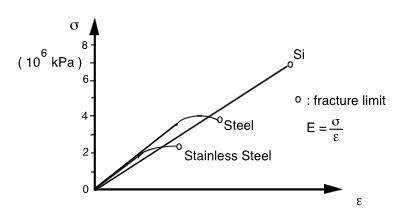
\includegraphics[width=0.95\textwidth,height=\textheight]{resistivity_Si.png}
\caption{image}
\end{figure}

Silicon is one of the favorite material since it is :

\begin{itemize}
\item
  Cheap, strong (and fragile)
\item
  0.001 - 20 \(k\Omega/cm\)
\item
  Stable oxide (\(SiO_2\)) pretty inert (wow)
\item
  various flavors of lattice, Silicon-Crystalline-Silicon, poly-silicon,
  amorphous silicon (unordered)
\end{itemize}

We can also use some GaAs, Quartz (which is just \(SiO_2\) with other
things), SiC, \(Al_2O_3\). On the figure
\protect\hyperlink{resistivity_Si}{{[}resistivity\_Si{]}}\{reference-type=``ref''
reference=``resistivity\_Si'': we can see how the Silicium can deform
under pressure and come back to its original shape without breaking for
large values. We can even make some wafer flexible using special
processes to make it extra thin.\\
We mostly use crystalline like Silicon even though non-crystalline have
become somewhat important in the industry. The doping plays a role
regarding the resistivity of the material.

\begin{figure}
\hypertarget{fig:resistivity-Si-Ohms}{%
\centering
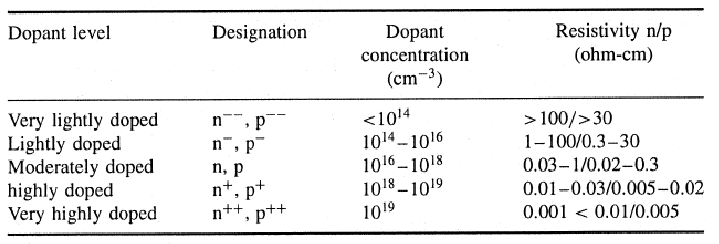
\includegraphics[width=0.75\textwidth,height=\textheight]{resistivity_Ohm_Si.png}
\caption{Resistivity for various doping
level}\label{fig:resistivity-Si-Ohms}
}
\end{figure}

r0.5
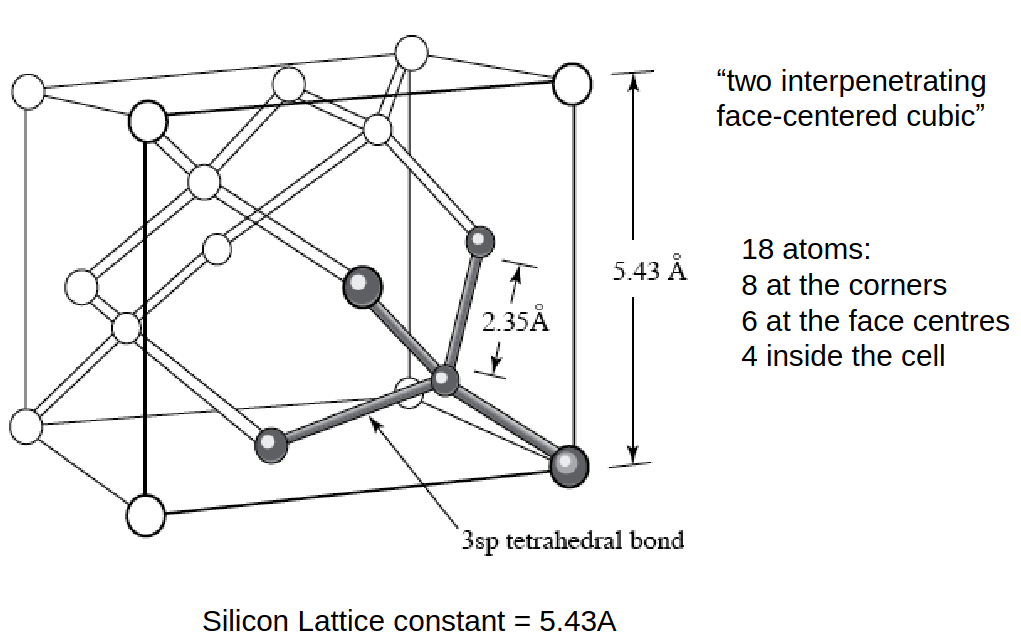
\includegraphics[width=0.95\textwidth,height=\textheight]{crystal_si.png}

Silicon atoms have \emph{4 valance electrons} and their \emph{covalent
bonds} are in a \emph{pryamid like structure} (\textbf{tetrahedron}).
For doping we can use :

\begin{itemize}
\item
  \ul{N-type :} use 5a group : Arsenic, Phosphorous, ...
\item
  \ul{P-type :} use 3a group : Boron, Gallium, Aluminum, ...
\end{itemize}

We have 4 atoms completely inside of a unit cell, the 8 ones on the
corner are shared with other cell (and count as 1 atom inside cell) and
the 6 remaining atoms on the faces are shared with 2 cells (count as 3
atoms inside cell). So we have \(4+1+3=8\) atoms inside the cell and the
cell volume is \((.543 nm)^3 = 1.6 \cdot10^{-22} cm^3\) which leads to a
density of \(\frac{8}{1.6 \cdot10^{-22} cm^3} = 5 \cdot 10^{22}\) atoms
\(/cm^3\).\\
To represent which angles we are viewing a cell, we are using the
\textbf{miller indices}. Different orientations of the lattice impact
the properties of the transistor due to different lattice form.

\hypertarget{miller-indices}{%
\subsubsection{Miller Indices}\label{miller-indices}}

To find the miller indices, we need to first draw a plane and see where
it intercepts with any x,y,z axis. If we only intercept the x axis at
\(a\) then we can write \([1 \quad 0 \quad 0]\) if we normalize \(a\) as
the \emph{cubic cell constant}.\\
We have various notation each with its own rule:

\begin{itemize}
\item
  \ul{\([100]\) :} \textbf{direction} in crystal coordinate
\item
  \ul{\(<100>\) :} set of \emph{symmetrically equivalent}
  \textbf{direction} in crystal coordinate
\item
  \ul{\((100)\) :} \textbf{plane} \emph{perpendicular} to a direction
\item
  \ul{\(\{100\}\) :} set of \emph{symmetrically equivalent}
  \textbf{plane} in crystal coordinate
\end{itemize}

To find the angle between two crystallographic directions we use the
equation with the two directions being \([h_1k_1l_1]\) and
\([h_2k_2l_2]\) :
\[cos(\theta) = \frac{h_1 h_2+k_1k_2+l_1l_2}{\sqrt{(h_1^2+k_1^2+l_1^2)(h_2^2+k_2^2+l_2^2)}}\]

\hypertarget{production-of-wafers}{%
\subsection{Production of wafers}\label{production-of-wafers}}

Single crystal silicon is one of the purest material made artifically
with a purity of \(99.999999999\) \%. We have a FCC lattices displaced
by \(.25\) Å in the 3 directions.

\begin{figure}
\hypertarget{fig:si-production-label}{%
\centering
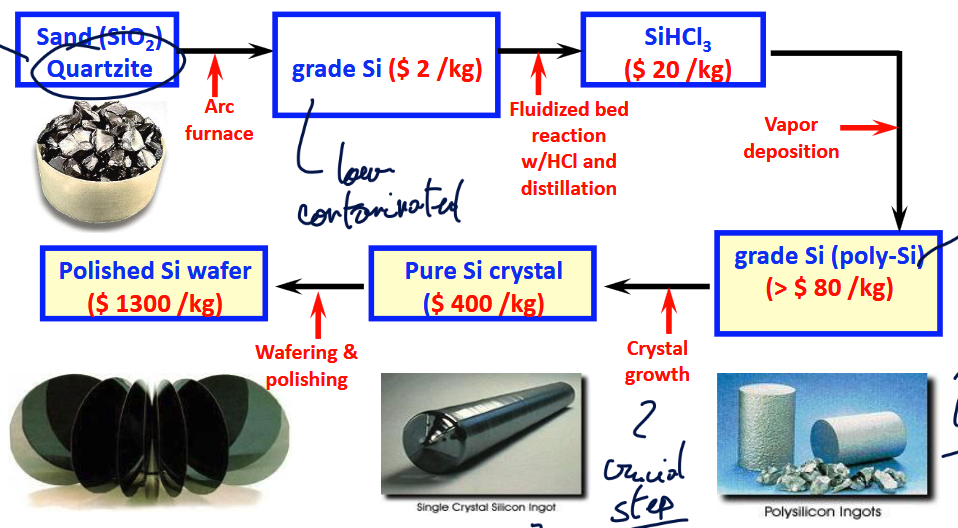
\includegraphics[width=0.75\textwidth,height=\textheight]{cycle_si.png}
\caption{Cycle of Si production}\label{fig:si-production-label}
}
\end{figure}

We can have some defect and non-idealities in the boule. Typically we
want a mono-crystalline structure where everything is ordered in the
same direction. But we can have :

\begin{itemize}
\item
  \ul{Polycrystalline :} multiple pockets named \textbf{grain} (or
  crystallites) where we find different direction of crystal
\item
  \ul{Amorphous :} unorganized structure and random
\end{itemize}

But first, we need to melt this \emph{quartz sand} with carbon at over
\(1900^\circ\)C. We have a purity of over \(98\) \%.

\hypertarget{wafer-processing}{%
\subsubsection{Wafer processing}\label{wafer-processing}}

\hypertarget{czochralski-pulling}{%
\paragraph{Czochralski Pulling}\label{czochralski-pulling}}

To create the big boule we then use to slice into wafers, we need to use
a specific machine. Typically, we need to use a \emph{seed crystal} with
a specific orientation which will make sure to give the same orientation
to the boule. We dip it and rotate in counter direction the pot and the
seed crystal. The rotation speed is important and the diameter is
\emph{inversely proportional to the pull rate}. The pull rate is in
\(mm/min\) and it takes a lot of time to produce just one boule. We need
30 hours to create a 2m boule and another 30 hours for heating and
cooling.\\

\hypertarget{slicing}{%
\paragraph{Slicing}\label{slicing}}

To indicate the orientation, we used to add a flat perpendicular to the
\(<110>\) direction but now we simply use a notch. We mostly use the
\(<100>\) with a precision of \(\pm 0.5^\circ\) and sometimes we use the
\(<111>\) with \(2^\circ-5^\circ\) off axis.\\
The cutting is done with wires coated with diamond and we have one
feeder spool and another one that takes the used wires.

\hypertarget{wafer-after-treatment}{%
\paragraph{Wafer after treatment}\label{wafer-after-treatment}}

\begin{enumerate}
\def\labelenumi{\arabic{enumi}.}
\item
  \textbf{Lapping} grind both sides, flatness around \(2-3 \mu m\),
  removes \(20\mu m\) per side.
\item
  \textbf{Edge Profiling}
\item
  \textbf{Etching} chemical etch to remove \emph{surface damage},
  removes \(20\mu m\) per side.
\item
  \textbf{Polishing} chemi-mechanical polish, using a slurry composed of
  \(Si O_2\) and some \(NaOH\), removes \(25\mu m\) per side. Nice
  mirror finish.
\item
  \textbf{Cleaning and Inspection}
\end{enumerate}

\hypertarget{crystal-orientations}{%
\paragraph{Crystal Orientations}\label{crystal-orientations}}

\begin{figure}
\hypertarget{fig:crystal-orientation-label}{%
\centering
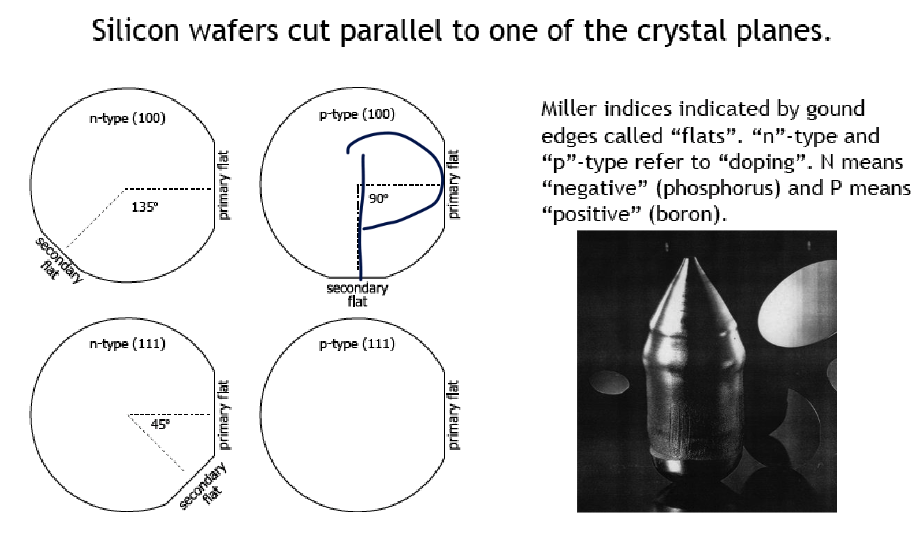
\includegraphics[width=0.75\textwidth,height=\textheight]{crystal_orientation.png}
\caption{Crystal orientation}\label{fig:crystal-orientation-label}
}
\end{figure}

r0.55
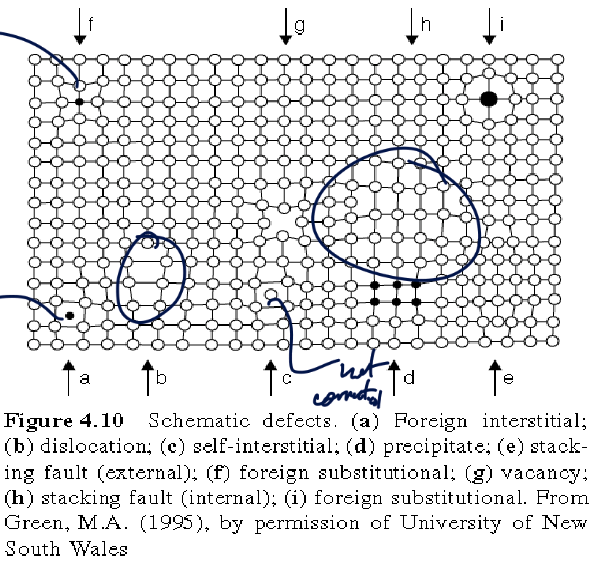
\includegraphics[width=0.95\textwidth,height=\textheight]{silicium_non_idealities.png}

But nowadays, we are using notches and not really using fully doped
wafer. We are doping locally the wafer. A notch indicates a \(<100>\)
n-type wafer.\\
We are processing the wafers in batches of 12 or 24 and they sit on a
glass tray (quartz boat) so the support doesn't melt. We will oxidize
the wafer to dope it which will tint the wafer. The color of the tint
can be used to see what type of doping it is and how doped it is using
some optics properties.\\
All those issues will lead to non-functional dies. We usually put some
dye on those to clearly and visually indicate if they are good or not.
We can't use the dies that are too close to the edge (\emph{edge
exclusion} 6 mm for 100-mm diameter wafers).\\
For this reason, we are wanting to use smaller chips to increase the
yield. There exists an ideal size that is related to the yield and
packaging cost. Now we have an optimum around \(13 cm^2\).

\hypertarget{packaging}{%
\paragraph{Packaging}\label{packaging}}

To do some packaging we need to dice the wafer, then use a pick and
place arm and finally add some wire (wire bonding) from the chip and its
pad to the housing of the chip.

\hypertarget{cleanroom}{%
\subsection{Cleanroom}\label{cleanroom}}

\begin{figure}
\hypertarget{fig:cleanroom-label}{%
\centering
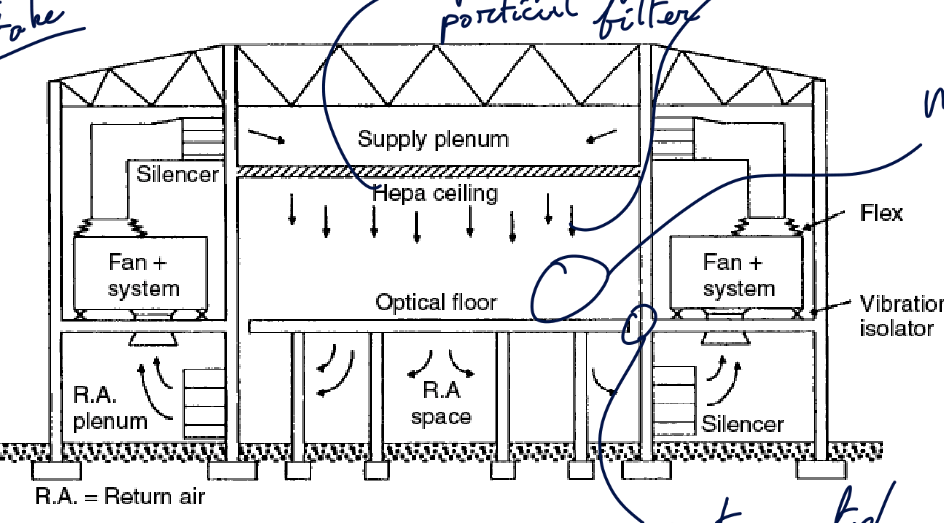
\includegraphics[width=0.7\textwidth,height=\textheight]{cleanroom.png}
\caption{Cleanroom}\label{fig:cleanroom-label}
}
\end{figure}

The purified air comes from the ceiling where it needs to go through
some \emph{HEPA} (High efficiency particulate air) filter in the
ceiling. We will usually only put one under the arrival of the air and
over the crucial equipment to reduce cost.\\
We have various class where each number indicates the amount of
particles \(>0.5\mu m\) in a cubic foot of air :

\begin{itemize}
\item
  Class 10000 : PCB, electronic packaging, medical devices
\item
  Class 1000 : MEMS, electronic packaging, hard disk drives
\item
  Class 100 : MEMS, RF/Photonic ICs
\item
  Class 10 : ICs
\end{itemize}

We also use the ISO standard :

\hypertarget{tab:my_label}{}
\begin{longtable}[]{@{}cccccccc@{}}
\caption{Comparison of ISO and FS209 standard}\tabularnewline
\toprule\noalign{}
Class & FS209 & 0.1 \(\mu m\) & 0.2 \(\mu m\) & 0.3 \(\mu m\) & 0.5
\(\mu m\) & 1 \(\mu m\) & 5 \(\mu m\) \\
\midrule\noalign{}
\endfirsthead
\toprule\noalign{}
Class & FS209 & 0.1 \(\mu m\) & 0.2 \(\mu m\) & 0.3 \(\mu m\) & 0.5
\(\mu m\) & 1 \(\mu m\) & 5 \(\mu m\) \\
\midrule\noalign{}
\endhead
\bottomrule\noalign{}
\endlastfoot
ISO1 & & 10 & 2 & & & & \\
ISO2 & & 100 & 24 & 10 & 4 & & \\
ISO3 & 1 & 1,000 & 237 & 102 & 35 & 8 & \\
ISO4 & 10 & 10,000 & 2,370 & 1,020 & 352 & 83 & \\
ISO5 & 100 & 100,000 & 23,700 & 10,200 & 3,520 & 832 & 29 \\
ISO6 & 1,000 & 1,000,000 & 237,000 & 102,000 & 35,200 & 8,320 & 293 \\
ISO7 & 10,000 & & & & 352,000 & 83,200 & 2,930 \\
ISO8 & 100,000 & & & & 3,520,000 & 832,000 & 29,300 \\
ISO9 & & & & & 35,200,000 & 8,320,000 & 293,000 \\
\end{longtable}

The cost in chips is due to the lithography where one chip can go
through 10 cycles and the more cycle we have the more expensive it is.

\hypertarget{lithography-photoresists-exposure-development}{%
\section{Lithography, photoresists, exposure,
development}\label{lithography-photoresists-exposure-development}}

When we do the lift-off we can either use \emph{positive} photo-resist
or \emph{negative} photo-resist. In positive, it is like usual, the
photo-mask is used to protect area that shouldn't be etched away. But
some compounds are not easy to etch. So sometimes, it is better to use
negative process to first deposit the photo-resist and then do the
blanket deposition of the compound. Then the lift-off is easy. We need
some special trapeze shape that lays on the smaller side for this
process.

\hypertarget{lithography-basic-steps}{%
\subsection{Lithography: basic steps}\label{lithography-basic-steps}}

The goal behind photolitography is to transfer a pattern into structure
in a thin layers. By repeating this operation multiple time we can
create some intricate and complex integrated circuits.

It mostly revolves around 3 major steps:

\begin{enumerate}
\def\labelenumi{\arabic{enumi}.}
\item
  \ul{Resist coating:} we deposit a light sensitive photoresist
\item
  \ul{Exposure:} we expose some part of it through a structural mask
\item
  \ul{Development:} we remove the photoresist
\end{enumerate}

Photoresist can be used in many many ways. When we etch away compounds
we usually have some \emph{undercut} which can be a structural problem.

\hypertarget{clean-wafer}{%
\subsubsection{Clean wafer}\label{clean-wafer}}

We first remove the particle with some rinsing in isopropanol,
ultrasonic and megasonic baths. To remove the organic particle we can
use some Piranha solution. To remove the metal traces that could diffuse
into the wafer, we can do some classic RCA clean, this step is needed
before high-temperature steps. RCA also removes ions that may be in the
substrate.

\hypertarget{rca-clean}{%
\paragraph{RCA-clean}\label{rca-clean}}

\begin{enumerate}
\def\labelenumi{\arabic{enumi}.}
\item
  Removal of the organic contaminants (organic + particle clean)
\item
  Removal of thin oxide layer (oxide strip, optional)
\item
  Removal of ionic contamination (ionic clean)
\end{enumerate}

\hypertarget{imec-clean}{%
\paragraph{IMEC clean}\label{imec-clean}}

The RCA-clean is quite an aggressive process and requires lot of
chenical products. The IMEC clean is a bit more nature friendly and uses
drying to force the particules to stay in the bath and not on the wafer.

\hypertarget{anti-reflective-coating-and-adhesion-promoter}{%
\subsubsection{Anti-reflective coating and adhesion
promoter}\label{anti-reflective-coating-and-adhesion-promoter}}

We use some Hexamethyldisilazane that will remove OH groups from the
surface making the wafer hydrophobic and thus photoresist-philic (since
photoresists are apolar).

\begin{enumerate}
\def\labelenumi{\arabic{enumi}.}
\item
  \textbf{TARC:} Top-side Anti Reflective Coating.

  \begin{itemize}
  \item
    Spin coated on top of photoresist
  \item
    Easier process
  \item
    Inferior performance
  \end{itemize}
\item
  \textbf{BARC:} Bottom side Anti-Reflective Coating.

  \begin{itemize}
  \item
    Deposited below photoresist layer
  \item
    Better performance
  \item
    Longer processing (plasma-etched)
  \end{itemize}
\end{enumerate}

\hypertarget{coat-with-photoresist}{%
\subsubsection{Coat with photoresist}\label{coat-with-photoresist}}

We can have positive or negative photoresist where:

\begin{itemize}
\item
  Positive: exposed area gets softer and easier to etch
\item
  Negative: exposed area gets harder and harder to etch
\end{itemize}

Spin coating is a process where we depose some droplets and spin the
wafer. Spinning it at a slow speed will spread the compound equally and
then we finish it off by spanning faster. It is a pretty good and
convenient way to coat a wafer's surface. But we can have some bumps
around the side of the wafer (edge bead) and the way steps are coated is
not always perfect.

\hypertarget{resist-spinning}{%
\paragraph{Resist spinning}\label{resist-spinning}}

We have some empirical equations for the thickness, and we spin with a
force of around 5 NM.

\[T = \frac{K \cdot C^\beta \cdot \eta^\gamma}{\omega^\alpha}\]

Where \(K\) is the calibration constant, \(C\) polymer concentration in
gram per 100 mL, \(\eta\) intrinsic viscosity, \(\omega\) rotation per
minute. The exponents are empirically determined.

We can also remove those edge bead in the process. But this doesn't
solve the issue of uneven coating around steps of the wafer.

\hypertarget{spray-coating}{%
\paragraph{Spray coating}\label{spray-coating}}

We have two nozzles where one will be used as the developer and the
other one is to rinse the wafer. It provides a smoother step coverage
and is widely used in MEMS devices.

\hypertarget{other-methods}{%
\paragraph{Other methods}\label{other-methods}}

We can also think about dip coating, laminating dry films of
photoresist, ...

\hypertarget{soft-bake}{%
\subsubsection{Soft Bake}\label{soft-bake}}

It is used to remove the solvents in the resist. It is non-sticky,
improves resolution, improves the strength of resist. But we shouldn't
bake too high too long or we would cause the embrittlement and make the
removal harder.

\hypertarget{exposure}{%
\subsubsection{Exposure}\label{exposure}}

There exists 5 exposure methods:

\hypertarget{lithography}{%
\paragraph{Lithography}\label{lithography}}

We expose the resist to UV light through a mask. We have to align the
mask precisely, it can be done manually for older technology. The
smaller we go the more expensive a mask is and we have more and more
layers.

\hypertarget{limits}{%
\paragraph{Limits}\label{limits}}

The main issue is the diffraction effects. Indeed, we have effects where
we could have some destructive or constructive waves that can be
unforseen. That's why some mask can have special patterns that will
result in the desired effect.

Those special patterns are Phase Shifting Mask where we will have some
special pattern to change the phase.

The process of making the wafer reflective can sometimes lead to create
some standing waves. Those standing waves can lead to uneven development
and rippled sidewalls. A solution for this is to use {arc} or post
exposure bake. This can also lead to linewidth variations due to
reflection.

\begin{figure}
\hypertarget{fig:enter-label}{%
\centering
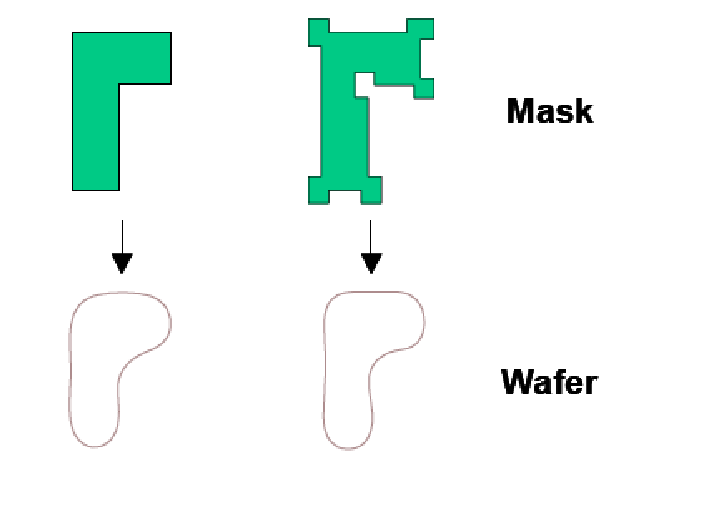
\includegraphics[width=0.5\textwidth,height=\textheight]{OPC.png}
\caption{Optical Proximity Correction}\label{fig:enter-label}
}
\end{figure}

\hypertarget{different-printing-techniques}{%
\subsubsection{Different printing
techniques}\label{different-printing-techniques}}

\begin{figure}
\hypertarget{fig:enter-label}{%
\centering
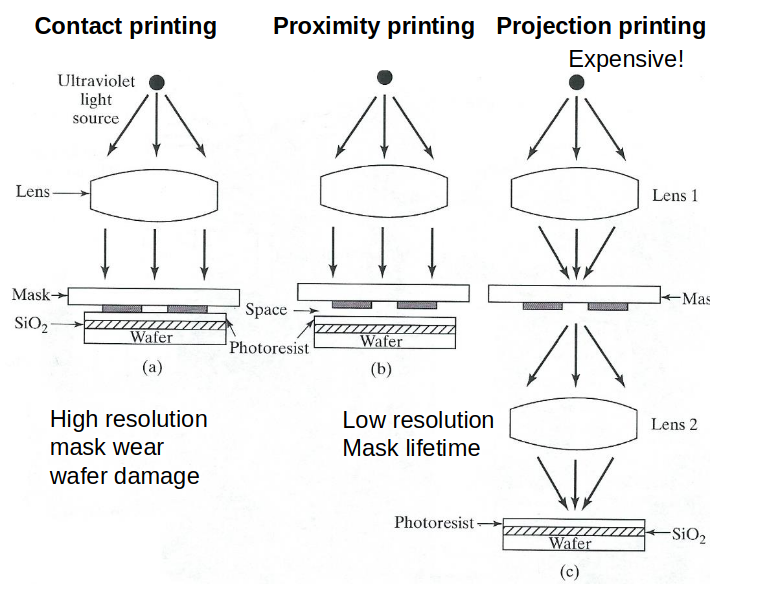
\includegraphics[width=0.65\textwidth,height=\textheight]{printing_techniques.png}
\caption{Printing techniques}\label{fig:enter-label}
}
\end{figure}

Usually we use stepper to print successively a pattern on the wafer.

\hypertarget{projection-printing}{%
\paragraph{Projection printing}\label{projection-printing}}

We concentrate and project on the wafer, There is a few key metrics such
as:

\begin{itemize}
\item
  \ul{Numerical Aperture:} \(NA = n sin(\theta)\)
\item
  \ul{Critical Dimension:} \(CD = kl \frac{\lambda}{NA}\)
\item
  \ul{Depth of Focus:} \(DOF = k_2 < 1\)
\end{itemize}

The depth of focus is an indicator to know when it is no longer good for
focus.

\begin{figure}
\hypertarget{fig:enter-label}{%
\centering
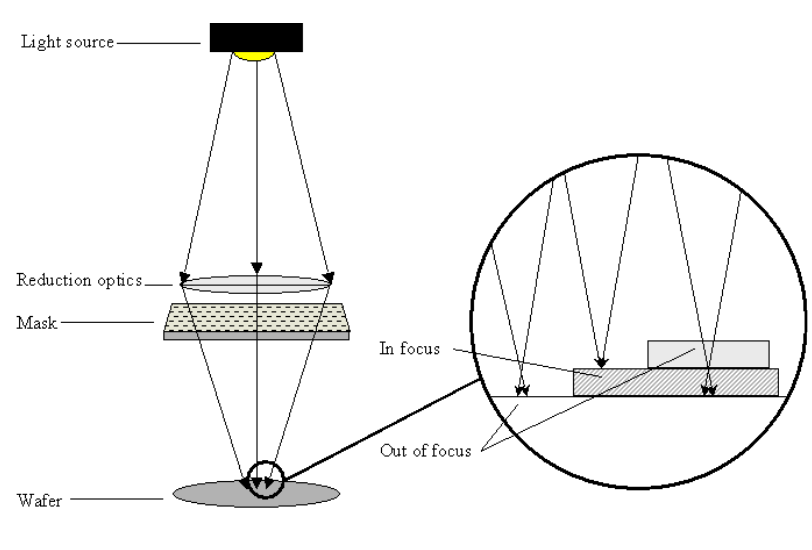
\includegraphics[width=0.5\textwidth,height=\textheight]{DOF_effects.png}
\caption{DOF effects}\label{fig:enter-label}
}
\end{figure}

\hypertarget{light-source}{%
\subsubsection{Light source}\label{light-source}}

Another important parameter we can play is the light source. Back then,
we used mercury bulbs for most lithographic work. It was a good enough
and pretty cheap UV source. But it would produce various line of UV. So
we had to use some filter to get only a specific wavelength.

\begin{longtable}[]{@{}lll@{}}
\caption{Wavelengths of light sources used in
photolithography}\tabularnewline
\toprule\noalign{}
\textbf{Source} & \textbf{Wavelength (nm)} & \textbf{Name} \\
\midrule\noalign{}
\endfirsthead
\toprule\noalign{}
\textbf{Source} & \textbf{Wavelength (nm)} & \textbf{Name} \\
\midrule\noalign{}
\endhead
\bottomrule\noalign{}
\endlastfoot
Hg arc lamp & 436 (blue) & g-line \\
& 405 (violet) & h-line \\
& 365 (UV) & i-line \\
& 248 & DUV \\
KrF excimer laser & 248 & DUV \\
ArF excimer laser & 193 & DUV \\
F\textsubscript{2} excimer laser & 157 & DUV (vacuum UV) \\
plasma & 13 & EUV (long x-ray) \\
\end{longtable}

The main attract to use lower wavelength light source is to be able to
draw better and smaller features. A good way to circumvent this rat race
is to use multiple mask to produce one result. So we can use multiple
ask with more spaced out features which simplifies amd relax constraints
of the problem.

\begin{enumerate}
\def\labelenumi{\arabic{enumi}.}
\item
  Double patterning: Litho-Etch-Litho-Etch (LELE)

  \begin{itemize}
  \item
    First technique introduced, reduces \(k_1\)
  \item
    More costly as it doubles the amount of mask, need a hard mask,
    possible overlay issues
  \end{itemize}
\item
  Double patterning: Self-Aligned Double Patterning (SADP)

  \begin{itemize}
  \item
    Solution to the overlay issue of LELE's masks self aligning
  \item
    Single lithography step, need to use an additional block or cut mask
    to remove unwanted material
  \item
    Complicated to design masks, process intensive
  \end{itemize}
\item
  Double patterning: Litho-Freeze-Litho-Etch (LFLE)

  \begin{itemize}
  \item
    Less complicated process than LELE, increased throughput, no need
    for hard mask.
  \item
    Dependent on development of freezing process, freezing cam cause
    issues in the lines.
  \end{itemize}
\item
  Double patterning: self-aligned quadruple patterning (SAQP)
\end{enumerate}

\hypertarget{euv}{%
\subsubsection{EUV}\label{euv}}

This is the hot new trend in the industry (ASML has the technology but
maybe huawei who knows). There has been prototypes since 2017 that can
do \(13.5\) nm and NA \(0.33\). It doesn't not have lenses but only
mirrors as we can't focus EUV light like this.

\hypertarget{issues}{%
\paragraph{Issues}\label{issues}}

We need to use some Bragg reflector that have an alternating thickness
of 2 nm of Mo and Si. It can only reflects \(70\%\) per mirror, so we
need a quite intense light source or we won't have anything coming to
the wafer.

\hypertarget{photo-vs-e-beam-lithography}{%
\paragraph{Photo vs E-beam
lithography}\label{photo-vs-e-beam-lithography}}

With E-beam lithography, we can be really accurate and not use any mask,
it comes at the disadvantage to slower processes. So we use E-beam to
create the mask for photo-lithography.

An issue is the scattering of the electron inside the wafer, it can also
go further than expected and in a random pattern.

\hypertarget{post-exposure-bake}{%
\subsubsection{Post exposure bake}\label{post-exposure-bake}}

It can help with wrinkles in the side wall. Baking can smooth things out
and is quite standard for positive resist. Can also enhance crosslinking
in negative resist.

\hypertarget{develop---wet-process}{%
\subsubsection{Develop - wet process}\label{develop---wet-process}}

Development is a wet chemical process as the wafer is immersed in
developer and rinsed and dried afterwards. We can also spray the
developer on the wafer as it spins but can be used and then dried. We
can use the spraying nozzle techniques.

\hypertarget{hard-bake}{%
\subsubsection{Hard bake}\label{hard-bake}}

Sometimes used to improve etch resistance of resist. But it can causes
the softer resists to reflow.

\hypertarget{etching-metal-deposition-ion-implantation-...}{%
\subsubsection{Etching, metal deposition, ion implantation,
...}\label{etching-metal-deposition-ion-implantation-...}}

See next chapters

\hypertarget{remove-photoresist}{%
\subsubsection{Remove photoresist}\label{remove-photoresist}}

To remove the pohotoresist, we can either go for wet etching with some
specialized solutions or acetone, NaOH, ...

We can also opt for O2 plasma etching.

\hypertarget{deposition-pvdacronym-labelpvd-acronym-formsingularshort-cvdacronym-labelcvd-acronym-formsingularshort-epitaxial-growth-ald}{%
\section{\texorpdfstring{Deposition: {[}pvd{]}\{acronym-label=``pvd''
acronym-form=``singular+short'': {[}cvd{]}\{acronym-label=``cvd''
acronym-form=``singular+short'': Epitaxial growth,
{ald}}{Deposition: {[}pvd{]}\{acronym-label=``pvd'' acronym-form=``singular+short'': {[}cvd{]}\{acronym-label=``cvd'' acronym-form=``singular+short'': Epitaxial growth, ald}}\label{deposition-pvdacronym-labelpvd-acronym-formsingularshort-cvdacronym-labelcvd-acronym-formsingularshort-epitaxial-growth-ald}}

To deposit a thin film layer we can use some {pvd} with evaporation or
sputtering. Another method is {cvd} that uses thermal, low pressure and
plasma enhanced (electrons stripped away from atoms).\\
With evaporation (heat + vacuum) we can reach a growth rate of
\(0.1-1 nm/s\). With sputtering (vacuum + plasma) we have a rate of
\(1-10nm/s\).

\hypertarget{pvd}{%
\subsection{\texorpdfstring{{pvd}}{pvd}}\label{pvd}}

\hypertarget{vacuum}{%
\subsubsection{Vacuum}\label{vacuum}}

r0.5
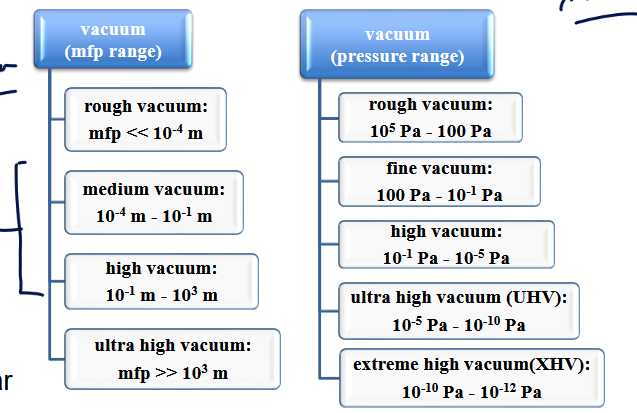
\includegraphics[width=0.95\textwidth,height=\textheight]{vacuum.png}

To realize deposition we need certain grade of vacuum. They are graded
based on their {mfp}. It indicates how far can a molecule travel before
hitting an other one. There is an equivalency between {mfp} and the
pressure in the environment.

The roughing pumps are simple a valve that rotates and will take out the
air. But it is not the purest form of vacuum.\\
High vacuum diffusion pump use some oil. The oil is heated up and will
vaporize, then when it gets cooled down it will take with them
molecules. The pressure at the bottom is higher and so we can simply use
a pump to take those extra molecules the oil vapor captured.

In a turbomolecular pump we are using some stator and rotor blades that
are inclined in such way that when a molecules strike the turbine blade
it will bounce and slowly travel to the bottom of the pump.

There is also cryogenic pump that is a mix of previously introduced
vacuum pumps.

\begin{figure}
\hypertarget{fig:PVD-label}{%
\centering
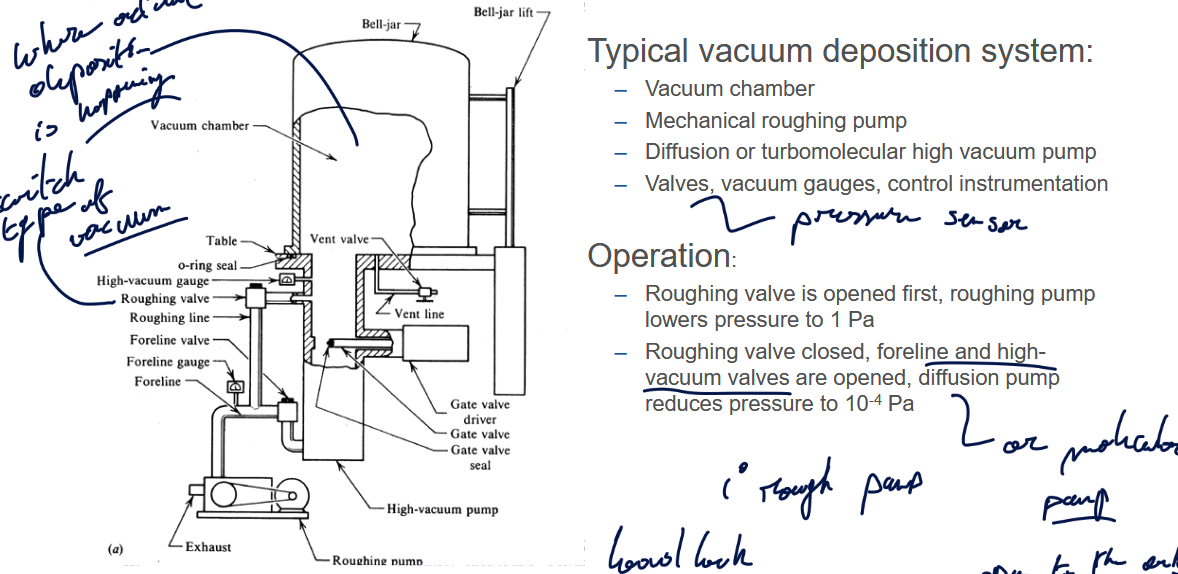
\includegraphics[width=0.75\textwidth,height=\textheight]{Vacuum_PVD.png}
\caption{Typical system for {pvd}}\label{fig:PVD-label}
}
\end{figure}

\hypertarget{pirani-gauge-10-3-mbar}{%
\paragraph{\texorpdfstring{Pirani Gauge (\(> 10^{-3}\)
mbar)}{Pirani Gauge (\textgreater{} 10\^{}\{-3\} mbar)}}\label{pirani-gauge-10-3-mbar}}

It is based on a \emph{weathstone bridge}. We will use a platinum wire
that is pretty linear and will get heat up, the way this heat transfer
occur depends on the pressure and is lower at lower pressure. So there
is a direct link with pressure, heat and finally resistor which is easy
to measure with such bridge.

\hypertarget{ion-gauge-10-2-mbar}{%
\paragraph{\texorpdfstring{Ion gauge (\(< 10^{-2}\)
mbar)}{Ion gauge (\textless{} 10\^{}\{-2\} mbar)}}\label{ion-gauge-10-2-mbar}}

The filaments will create a \emph{space-charge} of free electrons. The
electrons are attached by the positive grid and the collisions with the
gas atoms will create Ion which can be measured.

\hypertarget{evaporation}{%
\subsubsection{Evaporation}\label{evaporation}}

Now, we want to actually vaporize and create thin film on our wafer to
grow all sorts of oxide, metals, polysilicon, ... There is two ways to
do it :

\begin{enumerate}
\def\labelenumi{\arabic{enumi}.}
\item
  Resistance heating evaporation :

  \begin{itemize}
  \item
    We have the crucible (holder of the compound) and the target (wafer)
    that gets heated
  \item
    Only low melting temperature point metals (or it gets too hard)
  \end{itemize}
\item
  Electron beam evaporation :

  \begin{itemize}
  \item
    We use some electron beam to strike the material that will get
    \emph{sublimate} (not a melting)
  \item
    We cool the crucible down and it doesn't need to be as pure as with
    heated method
  \item
    Good for high melting point metals
  \end{itemize}
\end{enumerate}

\begin{figure}
\hypertarget{fig:evap-label}{%
\centering
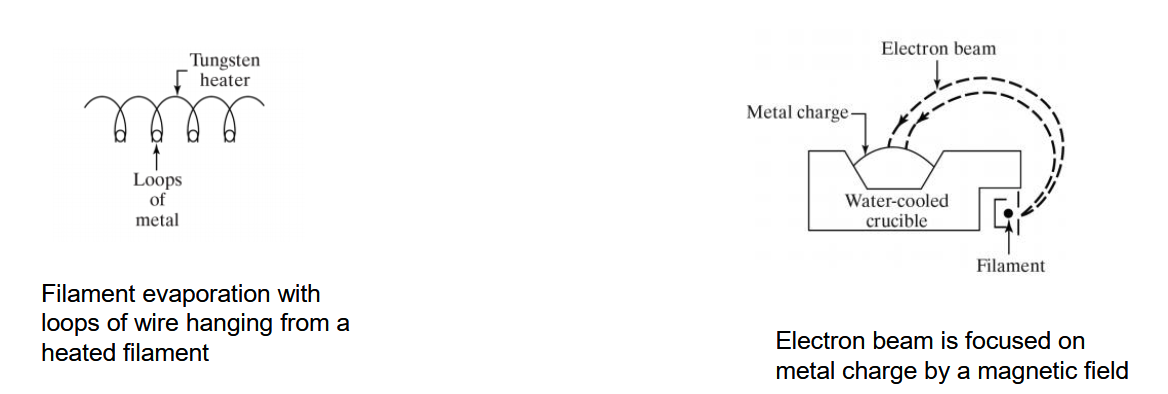
\includegraphics[width=0.85\textwidth,height=\textheight]{evaporation_method.png}
\caption{Evaporation techniques}\label{fig:evap-label}
}
\end{figure}

\hypertarget{coverage-issues}{%
\paragraph{Coverage issues}\label{coverage-issues}}

Due to the radiating pattern from the crucible to the target, we will
have discontinuity on the wafer which is not acceptable for traces or
oxide. So we will gently spin the target to slightly change the momentum
and so atoms will strike the sidewall. We also heat up the substrate to
further help the step coverage.

\begin{figure}
\hypertarget{fig:pvd-conf-label}{%
\centering
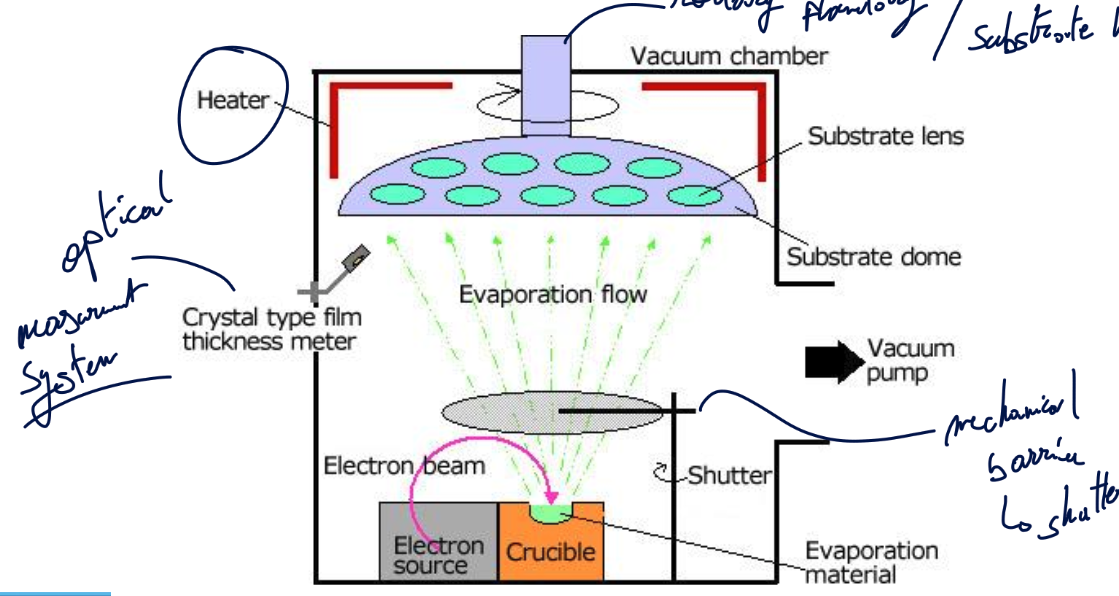
\includegraphics[width=0.5\textwidth,height=\textheight]{config_PVD.png}
\caption{Configuration for {pvd}}\label{fig:pvd-conf-label}
}
\end{figure}

\hypertarget{plasma}{%
\subsubsection{Plasma}\label{plasma}}

Plasma is a low pressure gas where a high energy field is used for
ionization creating a large number of ions and free electrons. So we rip
electrons of the nuclei and this happens in a vacuum. Plasma contains an
equal concentrations of ions and electrons. Electric potential is
approximately constant inside the plasma. We are using weak plasma so
mostly neutral atoms/molecules.

\begin{figure}
\hypertarget{fig:plasma-sputtering-label}{%
\centering
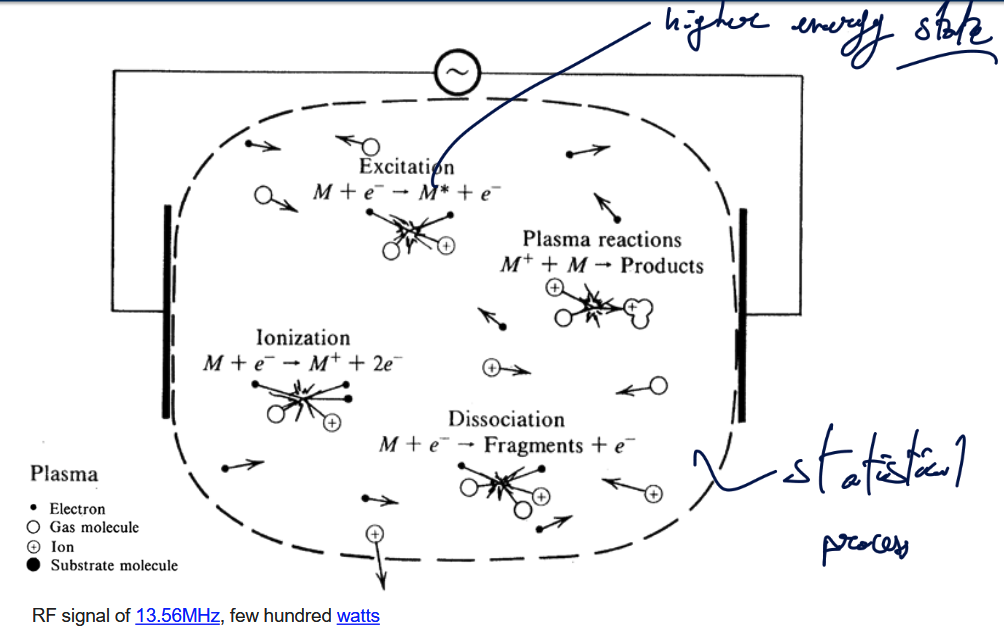
\includegraphics[width=0.51\textwidth,height=\textheight]{plasma.png}
\caption{Plasma using sputtering}\label{fig:plasma-sputtering-label}
}
\end{figure}

So the ions of the plasma will strike the target releasing them and
letting them go onto the wafer. We talk about a \textbf{sputtering
yield} which indicates
\(S = \text{\# of ejected target atoms} / \text{incoming ions}\) and it
is usually \(0.1<S<30\).\\
For example we can use a plasma of \(N_2\) and a \(Ti\) target that will
create a thin film layer of the substrate of \(TiN\).\\
Using sputtering can be quite beneficial especially for multi-components
thin-films. It is also better for lateral thickness uniformity. We have
a superposition of multiple point sources.

\hypertarget{cvd}{%
\subsection{\texorpdfstring{{cvd}}{cvd}}\label{cvd}}

The idea here is to use some chemical reaction to go from a gas phase to
a solid phase. Typically we will use a sort of boundary layer which will
trigger a reaction and deposit on the wafer. We need to remember that
\emph{natural} chemical reaction are trigger when we mix different
molecules that will reach a higher state of energy and will tend to a
lower state of energy. If we want to reverse this reaction we need to
give the same amount of lost energy.

\hypertarget{tab:deposition_methods}{}
\begin{longtable}[]{@{}llcl@{}}
\caption{Deposition methods, source gases, temperature, and
stability.}\tabularnewline
\toprule\noalign{}
\textbf{Material/method} & \textbf{Source gases} & \textbf{Temperature}
& \textbf{Stability} \\
\midrule\noalign{}
\endfirsthead
\toprule\noalign{}
\textbf{Material/method} & \textbf{Source gases} & \textbf{Temperature}
& \textbf{Stability} \\
\midrule\noalign{}
\endhead
\bottomrule\noalign{}
\endlastfoot
{lto} & SiH\(_4\) + O\(_2\) & 425\(^\circ\)C & Densifies \\
{hto} & SiCl\(_2\)H\(_2\) + N\(_2\)O & 900\(^\circ\)C & Loses Cl \\
{teos} & {teos} + O\(_2\) & 700\(^\circ\)C & Stable \\
{pecvd} OX & SiH\(_4\) + N\(_2\)O & 300\(^\circ\)C & Loses H \\
{lpcvd} poly & SiH\(_4\) & 620\(^\circ\)C & Grain growth \\
{lpcvd} a-Si & SiH\(_4\) & 570\(^\circ\)C & Crystallizes \\
{lpcvd} Si\(_3\)N\(_4\) & SiH\(_2\)Cl\(_2\) + NH\(_3\) & 800\(^\circ\)C
& Stable \\
{pecvd} SiN\(_x\) & SiH\(_4\) + NH\(_3\) & 300\(^\circ\)C & Loses H \\
CVD-W & WF\(_6\) + SiH\(_4\) & 400\(^\circ\)C & Grain growth \\
\end{longtable}

There is many chemical reactions showed in the course so check out page
40-45. When we grow an oxide or anything, we can either be \textbf{mass
transport limited} (velocity of the molecules saturate) or
\textbf{surface reaction limited} (the surface isn't heated enough and
the reaction isn't going well).

\hypertarget{reactor}{%
\subsubsection{Reactor}\label{reactor}}

\begin{figure}
\hypertarget{fig:cvd-reactors-label}{%
\centering
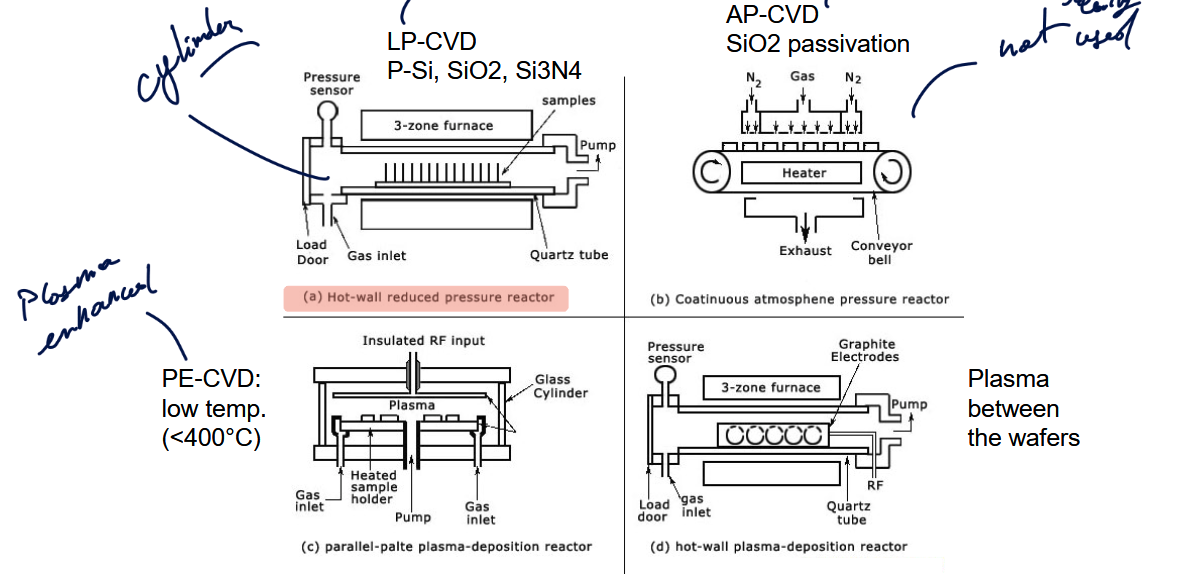
\includegraphics[width=0.85\textwidth,height=\textheight]{reactor.png}
\caption{CVD Reactors}\label{fig:cvd-reactors-label}
}
\end{figure}

\hypertarget{apcvd---atmospheric-pressure}{%
\paragraph{1. APCVD - Atmospheric
Pressure}\label{apcvd---atmospheric-pressure}}

It is pretty simple, we put the wafer on a conveyor belt that heats up
the wafer. We use some ozone and {teos} gas.

\hypertarget{lpcvd---low-pressure}{%
\paragraph{\texorpdfstring{2. {lpcvd} - Low
Pressure}{2. lpcvd - Low Pressure}}\label{lpcvd---low-pressure}}

We can stack the wafer vertically so keep them in the boat as we insert
them in the furnace. It needs a pressure of \(0.1-2\) Torr and it needs
high temperature and has a slow growth rate. It is ideal for batch
processing.

\hypertarget{pecvd---plasma-enhanced}{%
\paragraph{\texorpdfstring{3. {pecvd} - Plasma
Enhanced}{3. pecvd - Plasma Enhanced}}\label{pecvd---plasma-enhanced}}

We induce plasma in the gas by using some RF. We need some inert and
process gas and the wafer needs to spin and be heated. This result in
better step coverage and needs relatively lower temperature while having
a high deposition rate.

PECVD diagram

At higher temperature the deposition pattern will create bigger
"\emph{blobs}" compared to lower temperature deposition.

\hypertarget{epitaxial-growth}{%
\subsubsection{Epitaxial growth}\label{epitaxial-growth}}

r0.5
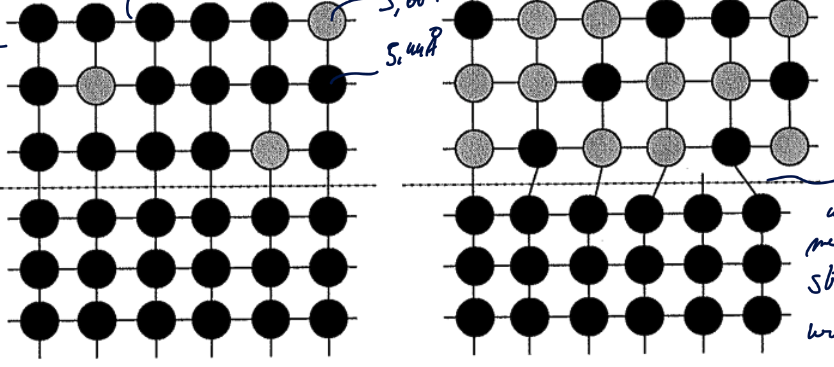
\includegraphics[width=0.95\textwidth,height=\textheight]{mechanical_stress_epitaxy.png}

We can grow some layer with the epitaxial technique. We can have :

\begin{itemize}
\item
  Homo-epitaxy : independent doping on a high-conductive substrate
\item
  Hetero-epitaxy : the difference in \(a\) size could create some
  mechanical stress
\end{itemize}

Some more advanced and recent epitaxy technique have been developed such
as {mbe}. With this new method we can deposit some complex stack of
material on our wafer. It is still in development and so there is not
yet a wide industry adoption of industrial workstation.

\hypertarget{ald}{%
\subsubsection{\texorpdfstring{{ald}}{ald}}\label{ald}}

With this method we can literally deposit \textbf{1 layer of molecules}
at a time ! We use some cycle consisting of a sequential precursor gas
pulses. It will produce a monolayer of gas on the substrate. Then a
second precursor gas is introduced which reacts with the monolayer and
will result into another monolayer on top.

\begin{figure}
\hypertarget{fig:ALD-pulsed-mode-label}{%
\centering
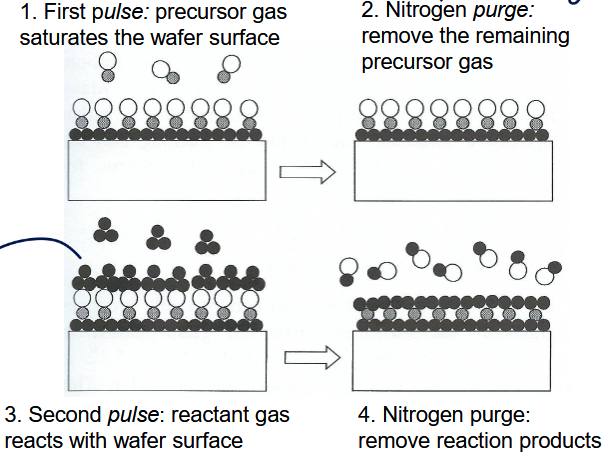
\includegraphics[width=0.65\textwidth,height=\textheight]{ALD_cycle.png}
\caption{{ald} process of pulsed mode}\label{fig:ALD-pulsed-mode-label}
}
\end{figure}

{ald} is a \emph{self-limiting} process so only one layer will be
deposited at a time. It is similar to {cvd} but we have 2 major steps to
diffuse the precursor gas not at the same time. We usually use Nitrogen
or Argon as a \emph{purge gas} which will "\emph{clean}" unwanted atoms.
This 2 cycles will help to avoid some \emph{parasitic} deposition like
in {cvd}.

It is also pretty good at making \emph{trenches} which is usually a FoM.
We usually compare width opening/depth. This value ranges from \(20\) to
\(100\).

\hypertarget{deposition-from-the-liquid-phase}{%
\subsubsection{Deposition from the liquid
phase}\label{deposition-from-the-liquid-phase}}

\hypertarget{electroplating-or-galvanic-deposition}{%
\paragraph{Electroplating or galvanic
deposition}\label{electroplating-or-galvanic-deposition}}

Thick conductor layers, high aspect ratio metallization. For this
method, we will use an anode and a cathode. We will use the reduction of
\(Cu\),\(Ni\) or \(Au\) typically onto the wafer (used as a cathode). We
have a pretty fast growth rate of \(0.1-10 \mu m/min\).

It is a good solution to create \emph{through-silicon vias} and do some
IC interconnects which is gaining more and more popularity lately.

\hypertarget{electroless-deposition}{%
\paragraph{Electroless deposition}\label{electroless-deposition}}

Selective metallization. We can have a growth rate of \(100nm/min\). For
intereconnect between IC we can use the \emph{damascene technique} :

\begin{figure}
\hypertarget{fig:enter-label}{%
\centering
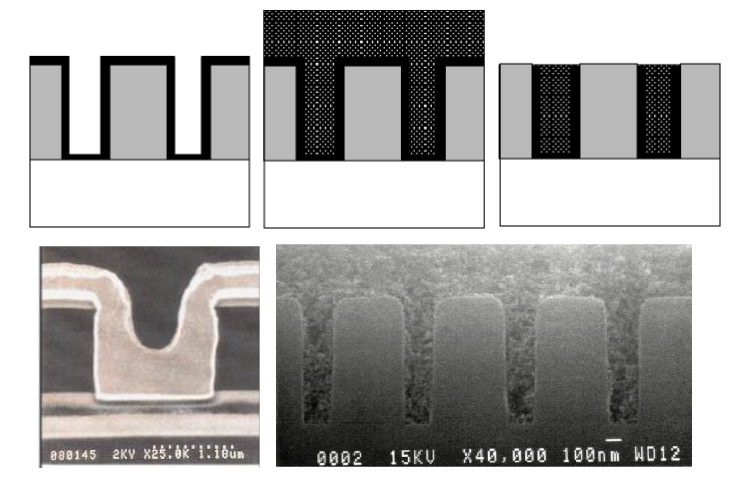
\includegraphics[width=0.5\textwidth,height=\textheight]{damascene_technique.png}
\caption{Damascene technique}\label{fig:enter-label}
}
\end{figure}

\hypertarget{spin-coating}{%
\paragraph{Spin coating}\label{spin-coating}}

Photoresists, thick polymer layers, spin-on glasses. Usually we start at
a slower speed to have the right amount of photoresist everywhere on the
glass then we finally spin it around \(5000 rpm\) which will cause
\emph{partial drying via evaporation}.

\hypertarget{sol-gel}{%
\paragraph{Sol-gel}\label{sol-gel}}

Porous dielectrics, thick and complex materials.

\hypertarget{measuring-the-thickness}{%
\subsection{Measuring the thickness}\label{measuring-the-thickness}}

To measure the thickness of the layer we can :

\begin{itemize}
\item
  Mechanical method : we use a needle that will check the thickness. It
  is not the most precise method.
\item
  Optical method :

  \begin{itemize}
  \item
    Reflectometry : we need the layer to not be totally opaque and we
    will measure the various wave that comes out of the wafer. We need
    to use small die and we can measure from \(10nm\) to \(50\mu m\).
  \item
    Elipsometry : it works with the polarization of light and can
    measure up to \(100\mu m\).
  \end{itemize}
\end{itemize}

\hypertarget{oxidation-wet-dry}{%
\section{Oxidation, wet, dry}\label{oxidation-wet-dry}}

r0.5
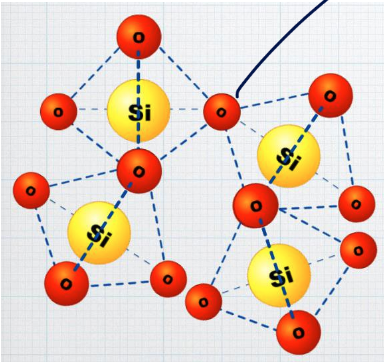
\includegraphics[width=0.95\textwidth,height=\textheight]{sio2_structure.png}

Sand is an abundant material that contains \(SiO_2\) or Silicon dioxide.
It is the main component of glass, optical fibers and we can find a
crystalline structure of \(SiO_2\) in quartz.

It has a \emph{tetrahedral arrangement} with one silicon bonded to four
oxygen atoms. We can see how most of oxygen atoms will be bonded with
\(Si\) atoms making the terahedra shape joined at corner. We call those
atoms the \emph{bridging atoms}. Not all oxygen atoms will be bonded to
two \(Si\), we call them the \emph{non-bridging atoms}. The density of
those non-bridging atoms determine the quality of the oxide.

They are not always aligned in such regular manner, it can be random
making some \emph{amorphous structure}. If there is no non-bridging
atoms, then

In microelectronic, we use thin layers of pure \(SiO_2\) and they are
amorphous. The density is about \(2-2.3 gm/cm^3\),
\(\varepsilon_r = 3.9\) (frequency dependent), \(n=1.5\) optical index.
The breakdown voltage is \(> 10^7 V/cm\) which is the main reason why we
need to lower \(V_{DD}\) as the thickness of the gate is getting
smaller.

But we will always have some traps at the interface which causes some
negative charges. The density of those defects is \(10^{11}cm^{-2}\), we
can even lower this value using some annealing process using hydrogen.
If we had more defects, this would result in a constant channel making
the material no longer semi-conducting.

We love silicon due to its abundance, good electrical property,
excellent insulating of its oxide, low defect at the interface.

\hypertarget{thermal-oxidation}{%
\subsection{Thermal oxidation}\label{thermal-oxidation}}

r0.5
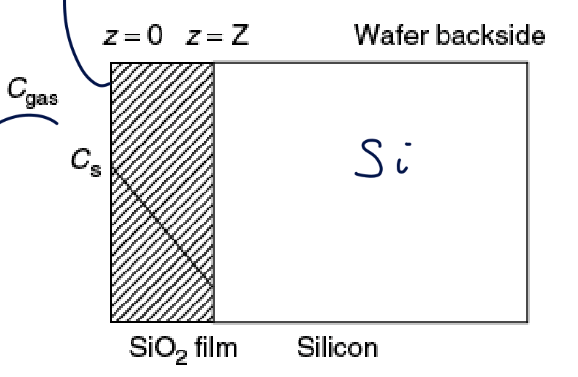
\includegraphics[width=0.95\textwidth,height=\textheight]{growth_of_oxide.png}

Silicium will naturally form an oxide and will grow a thin layer of it.
This process is only for \(Si\) and not present in other type of
semi-conductor such a \(GaAs\), \(Ge\), ... This oxide can be used as :

\begin{itemize}
\item
  Implant, diffusion mask
\item
  Surface passivation
\item
  Isolation between transistors
\item
  Key component of MOS structures
\item
  Dielectric for multilevel interconnect
\item
  Cleaning
\end{itemize}

As shown on the figure, the concentration of oxygen will reduce the
further we go towards the right which explains the slowing down of the
process. This will create a \textbf{consumption} effect where the oxide
will grow upwards and backwards. 1 mole of \(SiO_2\) is taking up more
volume than 1 mole of \(Si\). If we grow \(d\) thickness of oxide, we
will have \(0.46d\) of Si consumed.

\begin{itemize}
\item
  \(Si\) : \(2\cdot 10^{-23} cm^3\)
\item
  \(SiO_2\) : \(4.4\cdot 10^{-23} cm^3\) so about \(2.2\) times bigger
  than \(Si\). Expansion will go both ways.
\end{itemize}

\hypertarget{wet-and-dry}{%
\subsubsection{Wet and dry}\label{wet-and-dry}}

\[\begin{aligned}
    \text{Dry: }& Si + O_2 \rightarrow SiO_2 & \text{Wet: }& Si + 2H_2O \rightarrow SiO_2 + 2H_2
\end{aligned}\]

In \textbf{dry and wet} oxide growth, a higher temperature will lead to
thicker oxide growth. This growth will decrease as times grows since the
concentration of oxygen diminish. The growth rate is faster in \emph{wet
oxide} but it has lower quality which makes it easier to etch.

Since temperature plays a major role, we will have \textbf{oxidation
furnace} where our wafers loaded on quartz boat will slowly roll into
the furnace which has multiple temperature zone for better control.

\begin{itemize}
\item
  Dry: slower growth rate, better quality, better breakdown voltage
  (\(5-10MV/cm\)) better suited for gate using {ald}.
\item
  Wet: faster growth rate, lower quality, good for masking and
  interconnect dielectric.
\end{itemize}

For a growth of \(0.5\mu m\) of oxide at \(1200 C^\circ\) it takes
around 6 hours for dry and around 1 hour for wet oxidation.

\hypertarget{locos}{%
\subsubsection{\texorpdfstring{{locos}}{locos}}\label{locos}}

It is a process used for \emph{isolation between transistor}. We can
simply use \emph{patterned oxide} as the steps (the transistor) are too
high and we can't do spin coating or metallisation. Reduction of
topography by about \(56\%\).

To do some masking of oxide we can use \(Si_3N_4\) which grows slower
than \(Si\). But this technique will introduce some stress due to the
thermal expansion of nitrite being much higher than of \(Si\). We will
add between the substrate and the nitrite a small oxide called
\emph{pad-oxide} (\(SiO_2\)) as a stress release layer.

\begin{enumerate}
\def\labelenumi{\arabic{enumi}.}
\item
  We first add the pad-oxide of \(20-30nm\) and then finally the
  \(Si_3N_4\) of around \(100-200nm\).
\item
  Wet oxidation to grow the oxide, mechanical stress will cause a
  \emph{bird's beak} to form.
\item
  Remove the nitride with HF-dip to remove the \emph{oxynitrate} and
  then \(H_3PO_3\) (phosphorous acid) to etch nitrite.
\item
  Etching of pad-oxide with HF
\end{enumerate}

\hypertarget{sti-and-dti}{%
\subsubsection{\texorpdfstring{{sti} and
{dti}}{sti and dti}}\label{sti-and-dti}}

\hypertarget{sti}{%
\paragraph{\texorpdfstring{{sti}}{sti}}\label{sti}}

With this method we can avoid the \emph{bird's beak} phenomena. We can
do from about \(0.25 \mu m\) nodes without much stress. The process flow
is as follow :

\begin{enumerate}
\def\labelenumi{\arabic{enumi}.}
\item
  Anisotropic etching of \(Si\)
\item
  Thermal oxidation
\item
  Oxidation growth with {cvd} (using {teos} process)
\item
  {cmp} of oxide
\end{enumerate}

\hypertarget{sti-vs.-locos}{%
\paragraph{\texorpdfstring{{sti}
vs.~{locos}}{sti vs.~locos}}\label{sti-vs.-locos}}

\begin{itemize}
\item
  {sti}: The drawn width is almost the effective width. Can place
  transistor closer increasing the \emph{packing density}. We have a
  larger drive current for devices with same drawn width. Less
  topography.
\item
  {locos}: The drawn width is bigger than the effective width due to
  \emph{bird's beak}. To have the same drive current, we need wider
  transistor which diminish the packing density. Hard to do this process
  for sub \(0.5 \mu m\).
\end{itemize}

\hypertarget{doping}{%
\subsection{Doping}\label{doping}}

There is two main process for doping, either Thermal diffusion or Ion
implantation. The later one is more modern and we usually go for a mix
of those technique.

Doping relies on the idea to put some foreign atoms in the lattice,
either group V to negatively charge it (with an extra electron that is
free to roam) or with a group III atoms that will create a hole. It will
\emph{locally} create a charge difference. Watch out, we can have some
\emph{hole recombination} and so have useless mix of group V and III
that will just cancels each other.

For doping we can have:

\begin{enumerate}
\def\labelenumi{\arabic{enumi}.}
\item
  Diffusion, using some \emph{diffusion/doping mask}:

  \begin{itemize}
  \item
    Gas that will bombard the wafer, not straight path so can have
    border effect
  \item
    Coating will use a thin film and will also have border effect
  \end{itemize}
\item
  Ion implantation, also uses a \emph{diffusion/doping mask} but will be
  quite different.
\end{enumerate}

\hypertarget{diffusion}{%
\subsubsection{Diffusion}\label{diffusion}}

It is a common mechanic phenomena where we will have a material that
will search for stability and diffuse to reach a stable state.

\hypertarget{thermal-diffusion}{%
\paragraph{Thermal diffusion}\label{thermal-diffusion}}

This process happens at high temperature \(1000^\circ\) and when the
wafer get exposed to dopant material vapor. The \emph{upper limit} is
related to the \textbf{solid solubility}. The lower limit is of
\(10^{13}\).

One of the advantage of using silicon, is the fact that the doping level
will impact the resistance per square making it an easy material to
module the resistance of.

\hypertarget{diffusion-theory}{%
\paragraph{Diffusion Theory}\label{diffusion-theory}}

We have a diffusion \emph{flux} of \emph{impurities} in one dimension.
(We are always using x as the vertical direction of diffusion).

\[\begin{aligned}
    F &= - D \frac{\partial C(x,t)}{\partial x} & D &= D_0 exp\left( \frac{-E_{\alpha}}{kT} \right)
\end{aligned}\]

We have \(D\) that is the \emph{diffusion coefficient} in \(cm^2/s\).
\(C\) is the dopant concentration per unit volume. We have \(D_0\) that
is the diffusion coefficient in \(cm^2/s\) at infinite temperature and
\(E_\alpha\) is the activation energy in \(eV\).

At low concentrations of dopant in silicon (\(10^{12} - 10^{16} cm^3\))
can be seen as constant. With this simplification, we can easily solve
the equation, we also see that gold, coper, ... have high diffusion
coefficient which is why we tend to avoid such metal in the clean room.

If we do not have a source or sink of the impurity, we know that the
\emph{change in impurity concentration with time must equal the local
decrease of diffusion flux}:

\[\begin{aligned}
    \frac{\partial C}{\partial t} &= - \frac{\partial F}{\partial x} = \frac{\partial}{\partial x} \left( D\frac{\partial C(x,t)}{\partial x} \right) & \frac{\partial C}{\partial t} &=  D\frac{\partial^2 C(x,t)}{\partial x^2} \text{ if D cst}
\end{aligned}\]

There are 2 methods of diffusion:

\begin{enumerate}
\def\labelenumi{\arabic{enumi}.}
\item
  \ul{Constant-surface-concentration:} using vapor, we have a constant
  concentration of dopants at the surface.
\item
  \ul{Constant-total-dopant:} thin layer, we have constant amount of
  impurity at the surface.
\end{enumerate}

\hypertarget{constant-surface-concentration}{%
\paragraph{Constant-surface-concentration}\label{constant-surface-concentration}}

\[\begin{aligned}
    \text{Init: } C(x,0) &= 0 & C(0,t) &= Cs & C(\infty, t) &=0\\
    C(x,t) &= C_S erfc\left( \frac{x}{2\sqrt{Dt}} \right) & erfc(z) &= 1-erf(z) & erf(z)&=\frac{2}{\sqrt{\pi}}\int_0^\pi e^{-y^2} dy
\end{aligned}\]

We have \(\sqrt{Dt}\) that is called the \emph{diffusion length} in
\(cm\). The total number of dopant atoms per unit area that has diffused
into the semiconductor is given by:

\[Q(t) = \int_{0}^\infty C(x,t) dx = \frac{2}{\sqrt{\pi}} C_s \sqrt{Dt} \approx 1.13 C_s \sqrt{Dt}\]

\hypertarget{constant-total-dopant}{%
\paragraph{Constant-total-dopant}\label{constant-total-dopant}}

\[\begin{aligned}
    C(x,0) &= 0 & \int_0^\infty C(x,t) dx &= \phi & C(\infty, t) &= 0\\
     & & C(x,t) &= \frac{\phi}{\sqrt{\pi D t}} exp \left( - \frac{x^2}{4 D t} \right)
\end{aligned}\]

Where \(\phi\) is the \emph{total amount of dopant} per unit area. So
the surface concentration (\(x=0\)) is \(\phi / \sqrt{\pi Dt}\).

We usually use those two methods and we call this a \emph{two step
diffusion process}. a pre-deposition diffused layer is first formed
using constant-surface-concentration condition. Then a drive-in (or
redistribution) diffusion is used using constant-total-dopant condition.

For most practical cases the diffusion length for the pre-deposition
stage is much smaller than the diffusion length of the drive-in
diffusion. This allows to make deep junctions, e.g.~for wells for CMOS.

\hypertarget{advanced-diffusion-theory}{%
\paragraph{Advanced Diffusion Theory}\label{advanced-diffusion-theory}}

We are oversimplifying the problem which will gives us incorrect values
when compared with reality. Moreover, the atoms vibrate and there is a
non-zero chance that a silicon atom moves from its lattice site which
will leave a vacancy.

Dopants diffuse in combination with silicon interstitials or vacancies
and the diffusion coefficient is therefore strongly influenced by the
concentration of interstitials or vacancies.

\hypertarget{high-doping-concentration-diffusion}{%
\paragraph{High Doping Concentration
Diffusion}\label{high-doping-concentration-diffusion}}

Here, our simple theory doesn't hold anymore. The diffusion profile is
different. Moreover, the diffusion of phosphorous at high concentration
is \emph{anomalous}. We often notice a \emph{kink} on the doping
profile. Then we have a deep tail region that extends further in the
doping region.

The anomalous diffusion behavior has been explained by the dissociation
of the phosphorus-vacancy pair (P+V2-) into P+, V- and an electron. The
singly charged acceptor vacancies (V-) enhance the diffusivity in the
tail region (by a factor of 100 at \(1000^\circ\)). So it is good for
creating deep n-type junction. Arsenic is preferred over phosphorous.

\hypertarget{tab:doping_levels}{}
\begin{longtable}[]{@{}lccc@{}}
\caption{Doping levels, designations, concentrations, and
resistivities.}\tabularnewline
\toprule\noalign{}
\textbf{Dopant level} & \textbf{Designation} & \textbf{Dopant
concentration} (cm\(^{-3}\)) & \textbf{Resistivity n/p} (ohm-cm) \\
\midrule\noalign{}
\endfirsthead
\toprule\noalign{}
\textbf{Dopant level} & \textbf{Designation} & \textbf{Dopant
concentration} (cm\(^{-3}\)) & \textbf{Resistivity n/p} (ohm-cm) \\
\midrule\noalign{}
\endhead
\bottomrule\noalign{}
\endlastfoot
Very lightly doped & n\(^{--}\), p\(^{--}\) & \(<\)10\(^{14}\) &
\(>\)100/\(>\)30 \\
Lightly doped & n\(^{-}\), p\(^{-}\) & 10\(^{14}\)--10\(^{16}\) &
1--100/0.3--30 \\
Moderately doped & n, p & 10\(^{16}\)--10\(^{18}\) &
0.03--1/0.02--0.3 \\
Highly doped & n\(^{+}\), p\(^{+}\) & 10\(^{18}\)--10\(^{19}\) &
0.01--0.03/0.005--0.02 \\
Very highly doped & n\(^{++}\), p\(^{++}\) & 10\(^{19}\) &
0.001\(<\)0.01/0.005 \\
\end{longtable}

Here, we are always talking in \(\Omega / cm\) resistance that relates
to the sheet resistance.

For diffusion we can either have diffusion through substitutional or
interstial diffusion.

\hypertarget{using-sio_2-for-masking}{%
\paragraph{\texorpdfstring{Using \(SiO_2\) for
masking}{Using SiO\_2 for masking}}\label{using-sio_2-for-masking}}

The diffusion of \(B,P,As\) in \(SiO_2\) is at least one order of
magnitude lower than in \(Si\). There exists some table that indicates
the thickness of the oxide for the diffusion of a given material at a
given temperature during a definite amount of time.

By mixing impurities, we can slowly diffuse some up to a deep depth and
then diffuse another type. They will cancel each other out which will
create some junction and deeper junction.

\begin{figure}
\hypertarget{fig:SDS-label}{%
\centering
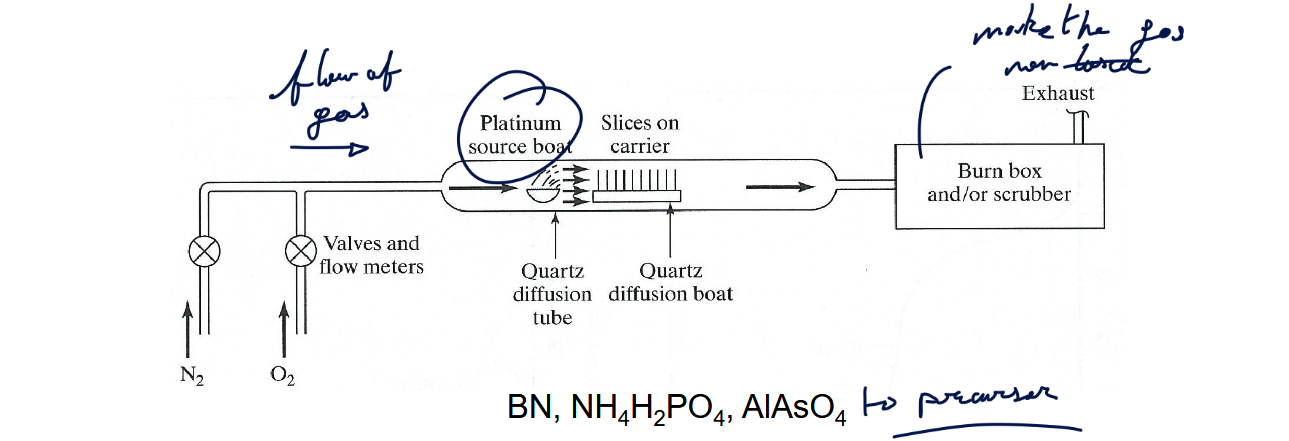
\includegraphics[width=0.75\textwidth,height=\textheight]{solid_dopant_sources.png}
\caption{Solid Dopant Sources}\label{fig:SDS-label}
}
\end{figure}

The boat we are using has some Boron nitride wafers between 2 substrate
wafers to diffuse it.

There is also a version that uses liquid dopant sources which is similar
to the solid dopant one except the \(N_2\) will be bubbling in the
bubbler. We can also have the same with gas using some dopant gas. We
have to add some scrubber system to trap all of the gases.

\hypertarget{ion-implantation-deposition-drive-in-and-rta}{%
\subsection{Ion implantation: deposition, drive-in and
RTA}\label{ion-implantation-deposition-drive-in-and-rta}}

\begin{figure}
\hypertarget{fig:ion-implanter-label}{%
\centering
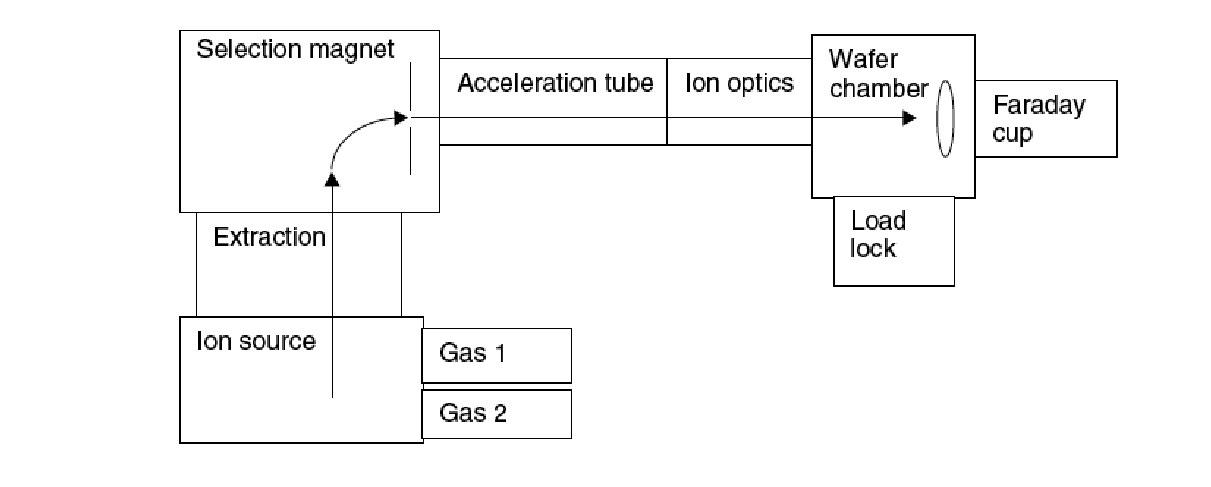
\includegraphics[width=0.75\textwidth,height=\textheight]{ion_implantation.png}
\caption{Basic elements of an
ion-implanter}\label{fig:ion-implanter-label}
}
\end{figure}

\begin{enumerate}
\def\labelenumi{\arabic{enumi}.}
\item
  \ul{\textbf{Ion source:}} it works at high voltage \(25 kV\) and
  creates a plasma with the desired impurity.
\item
  \ul{\textbf{Mass spectrometer:}} it will selects which ion we want in
  this right angle bend.
\item
  \ul{\textbf{High voltage accelerator column:}} to make it faster we
  accelerate it with a field of over \(5MeV\).
\item
  \ul{\textbf{Scanning system:}} to deposit the right amount, we also
  make it slightly bend so the neutral particles will go straight and
  not hit the wafer.
\item
  \ul{\textbf{Target chamber:}} operated in vacuum conditions and is
  where the wafer is located in.
\end{enumerate}

Something important to note is the fact that the ions will hit the wafer
pretty straight but it will go through a random path in the wafer. This
will lead to a gaussian distribution of the particles around a certain
depth.

\[N(x) = N_p exp \left( - \frac{(x-R_p)^2}{2 \Delta R_p^2} \right) \qquad N_p = \frac{\phi}{\sqrt{2 \pi} \Delta R_p}
    \label{eq:ion}\]

\hypertarget{ion-implantation}{%
\subsubsection{Ion implantation}\label{ion-implantation}}

So the main idea is "simply" accelerating ions pretty quickly so that
they will penetrate inside the wafer up to a few tenths of microns. Of
course, masking is used so we can create the desired pattern and not
simply bombard the full wafer. We can either use some silicon dioxide or
photoresist.

In \protect\hyperlink{eq:ion}{{[}eq:ion{]}}\{reference-type=``ref''
reference=``eq:ion'': \(\phi\) is the \emph{ion dose per unit area} and
\(R_p\) is the distance to the peak from the surface and is called the
\emph{projected range}. \(\Delta R_p\) is the \emph{projected straggle}
is the distance from the peak where the concentration is reduced by
\(40\%\) and is usually empirical.

One major advantage and use case of ion implantation is to put some ions
below a gate oxide for example. But we damage the lattice by bombarding
like this and we require some \textbf{annealing} at \(900^\circ\) to
repair the damage. If we go even hotter we can do some \emph{drive-in}
to diffuse even further the dopant into the silicon.

\hypertarget{masking}{%
\subsubsection{Masking}\label{masking}}

Now, how thick should a mask be so all the ions will be trapped inside
the mask ? But it is important to note that since it is a Gaussian
distribution we will always have a probability that the ions will go
inside the substrate.

Something that is even more annoying is the fact that we will have some
ions around a slit that will go under the mask.

\begin{figure}
\hypertarget{fig:implantation-label}{%
\centering
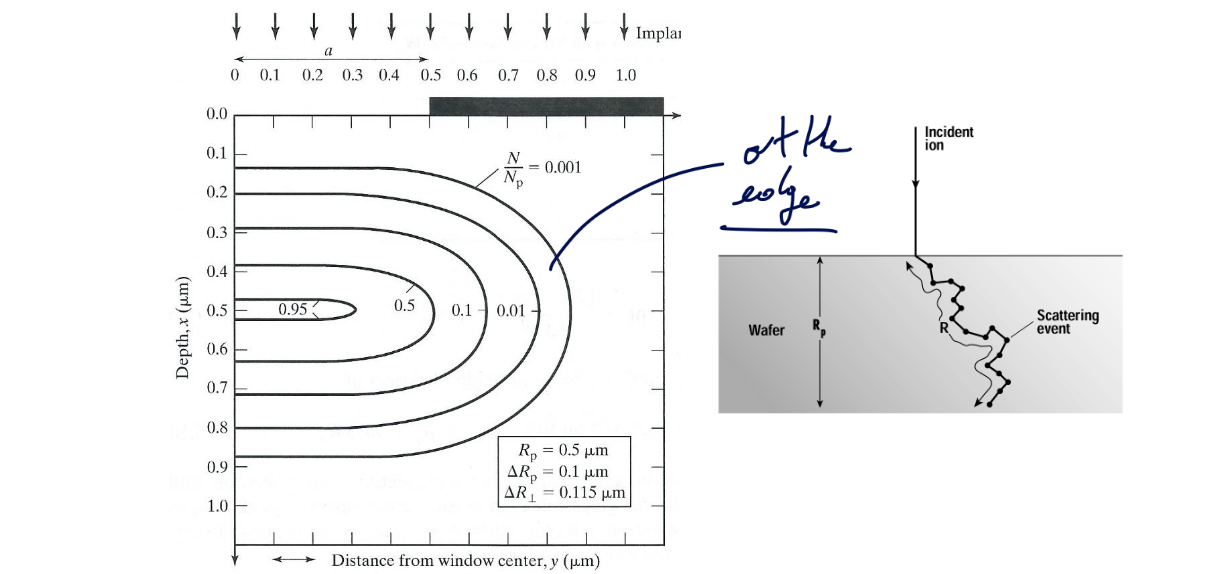
\includegraphics[width=0.75\textwidth,height=\textheight]{implanatation.png}
\caption{Ion Implantation}\label{fig:implantation-label}
}
\end{figure}

We have to realize some empirical experiments to see under which
condition a given ions will dope or not the silicon or stop at the
silicon dioxide.

\hypertarget{annealing}{%
\subsubsection{Annealing}\label{annealing}}

It is a crucial step after doing some ion implantation where we have to
restore the lattice from any damages. But it also allows the dopants to
take the correct spot inside the lattice.

As hinted previously, doing this sort of baking at high temperature will
lead to some \emph{drive-in} by diffusion and we will have more spread.

\hypertarget{rta}{%
\paragraph{\texorpdfstring{{rta}}{rta}}\label{rta}}

To avoid this diffusion to happen to fast, we can use some lighting bulb
to produce a quick and rapid heating of the substrate.

\hypertarget{channeling}{%
\subsubsection{Channeling}\label{channeling}}

One thing that can happen if we have a perfect lattice is the fact that
an ion may not bounce and will went through the lattice directly. So
instead of having a nice gaussian we will see some odd shapes and
multiple peaks.

\hypertarget{solutions}{%
\paragraph{Solutions}\label{solutions}}

We can add a layer of oxide so it will force the ions to bounce around.
Or we can tilt the wafer or even grow some \emph{amorphous} Poly-Si.

\hypertarget{profile-verification}{%
\subsubsection{Profile Verification}\label{profile-verification}}

After applying a layer, we would like to measure the thickness of an
oxide or other things:

\begin{itemize}
\item
  \ul{{sims}}
\item
  \ul{{srp}:} destructive process since we bombard the surface and
  measure the amount of ions and neutral particules.
\end{itemize}

There is also electrical measurement where we use two probes and measure
the resistivity by applying a current. This will leave some \emph{damage
craters} due to the probing. There is another version that uses 4 probes
that measures the current and the voltage.

\hypertarget{etching-wet-dry-plasma-drie}{%
\section{Etching, wet, dry, plasma,
DRIE}\label{etching-wet-dry-plasma-drie}}

In etching, we distinguish two types:

\begin{itemize}
\item
  Isotropic: the etching goes in every direction and etches pretty
  equally

  \begin{itemize}
  \tightlist
  \item
    Plasma, Wet (mostly), {rie}
  \end{itemize}
\item
  Anisotropic: the etching prefers one orientation of the lattice

  \begin{itemize}
  \tightlist
  \item
    Plasma, {[}rie{]}\{acronym-label=``rie''
    acronym-form=``singular+short'': Ion milling,
    {[}drie{]}\{acronym-label=``drie'' acronym-form=``singular+short'':
    KOH wet
  \end{itemize}
\end{itemize}

\hypertarget{wet-etching}{%
\subsection{Wet Etching}\label{wet-etching}}

\hypertarget{isotropic}{%
\subsubsection{Isotropic}\label{isotropic}}

To keep a constant gradient locally, we have to replace all the time the
solution that's why we overflow the bath by adding continuously new
etchant and uses a stirer.

Because of the way wet etching works, we will have \textbf{undercut
area} that we also call \emph{etch bias} and can be an issue for
features that are too close to each other. Below \(3 \mu m\) we will
prefer dry etching.

To stop precisely and quickly the reaction, we use a a trap at the
bottom of the bath to quickly dump the etchant and we spray the wafer
with solution to stop quickly and precisely the process.

\begin{longtable}[]{@{}ll@{}}
\caption{Etchants for various materials}\tabularnewline
\toprule\noalign{}
\textbf{Material} & \textbf{Etchant} \\
\midrule\noalign{}
\endfirsthead
\toprule\noalign{}
\textbf{Material} & \textbf{Etchant} \\
\midrule\noalign{}
\endhead
\bottomrule\noalign{}
\endlastfoot
SiO\(_2\) & \(NH_4F:HF \ (7:1)\) BHF, \(35^\circ C\) \\
SiO\(_2\) & \({NH_4F:CH_3COOH:C_2H_6O_2:H_2O} \ (14:32:4:50)\) \\
poly-Si & \({HF:HNO_3:H_2O} \ (6:10:40)\) \\
Al & \({H_3PO_4:HNO_3:H_2O} \ (80:4:16)\), \\
& water can be changed to acetic acid \\
Mo & \({H_3PO_4:HNO_3:H_2O} \ (80:4:16)\) \\
W, TiW & \({H_2O_2:H_2O} \ (1:1)\) \\
Cr & \({Ce(NH_4)NO_3:HNO_3:H_2O} \ (1:1:1)\) \\
Cu & \({HNO_3:H_2O} \ (1:1)\) \\
Ni & \({HNO_3:CH_3COOH:H_2SO_4} \ (5:5:2)\) \\
Ti & \({HF:H_2O_2}\) \\
Au & \({KI:I_2:H_2O}\); \({KCN:H_2O}\) \\
\end{longtable}

We can also use other etchant or use some HF that is often used for
\(SiO_2\). But HF is pretty dangerous to handle as a spill on your skin
doesn't burn or causes pain immediately, it will slowly penetrate the
body until it attacks the bone.

\hypertarget{anisotropic}{%
\subsubsection{Anisotropic}\label{anisotropic}}

We also have some anisotropic wet etchant where we will have various
effect depending on the lattice orientation (using the notation as seen
previously):

\begin{figure}
\hypertarget{fig:enter-label}{%
\centering
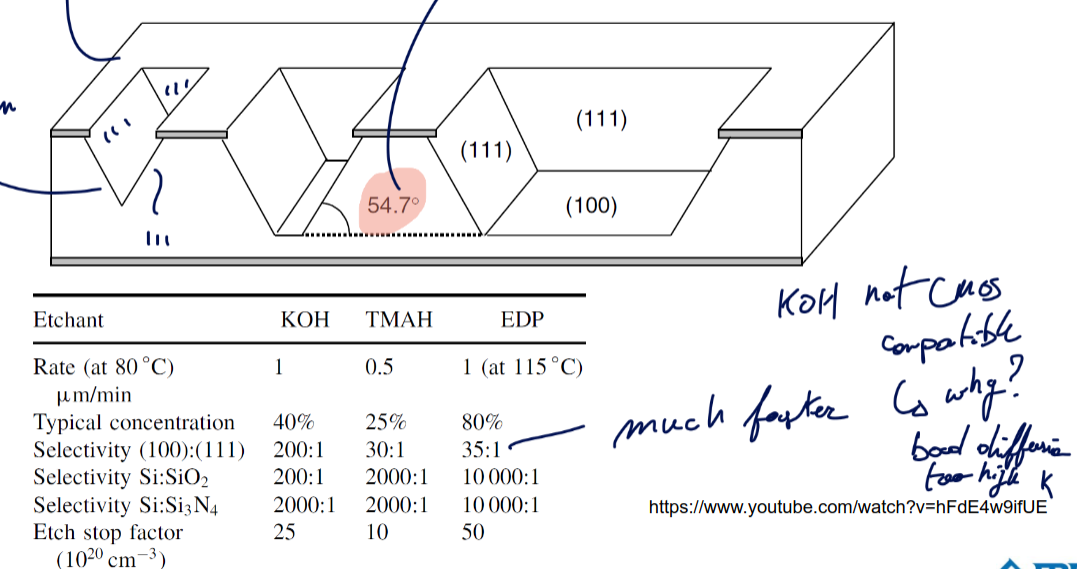
\includegraphics[width=0.75\textwidth,height=\textheight]{ansitropic_wet.png}
\caption{Anisotropic wet etching}\label{fig:enter-label}
}
\end{figure}

\hypertarget{dry-etching}{%
\subsection{Dry Etching}\label{dry-etching}}

This process comes in many flavors but they are all a combination of
some excitation energy and pressure where we either have high energy-low
pressure or low energy-high pressure. We use mechanical and chemical
aswell to better control the process.

\begin{itemize}
\item
  Physical: we bombard the wafer with some \emph{positive ions} and we
  strike the substrate with high kinetic energy.
\item
  Chemical: we can either use neutral or ionized species to react with
  the surface to create some \emph{volatile product}. This process is
  often \emph{isotropic}.
\end{itemize}

\hypertarget{plasma-etching}{%
\subsubsection{Plasma Etching}\label{plasma-etching}}

Plasma is a \emph{fully or partially} ionized gas containing an equal
amount of positives and negatives charges but has different number of
unionized molecules. We then need a strong enough electrical field to
ionize the gas.

The goal of plasma etching is to produce some chemically reactive
species from a relative inert gas. Then we make this gas react with the
specific material we want to etch and the product should be pretty
volatile to be easily removed. We need high speed and high chemical
reactions between neutrals and the substrate materials. We use a
\emph{carrier} gas producing some ions and reactive neutrals. This
reactive neutrals attack the sidewall and the normal surface. BUT, the
positive ions will \textbf{only} attack the normal surface. So we will
first go in the vertical direction.

We have around \(10^{15} cm^{-3}\) and \(10^8-10^{12} cm^{-3}\). After
hitting the surface, we may have the volatile particles to react against
the wall of the chamber which is really problematic. But washing is not
always the solution as it can disrupt the precise setting for the
reaction to happen at an optimal point.

To have some idea about the type of gases we can use look at the various
tables chapter 5 page 30-32.

\hypertarget{ion-milling---drie}{%
\subsubsection{\texorpdfstring{Ion milling -
{drie}}{Ion milling - drie}}\label{ion-milling---drie}}

Ion milling is a sort of \emph{sputter etching} where the wafer is
coupled to a voltage source. It also uses some plasma gas but the added
voltage to the wafer add some acceleration to the positive ions.

\begin{figure}
\hypertarget{fig:rie-setup-label}{%
\centering
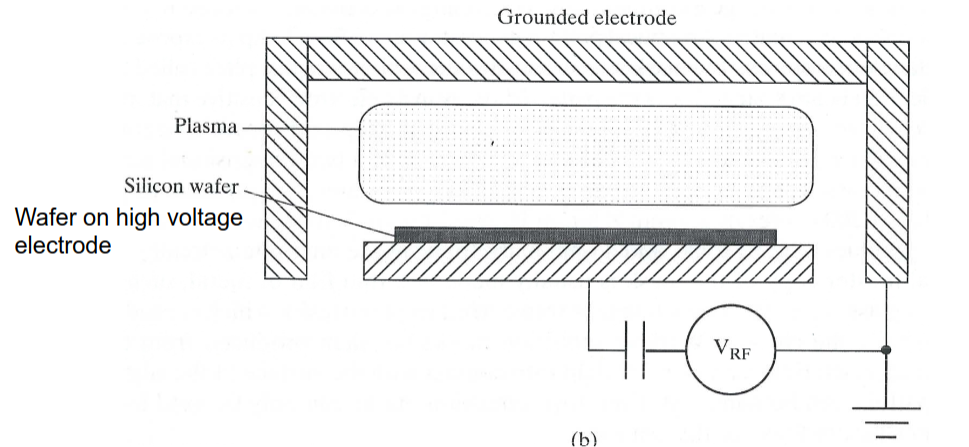
\includegraphics[width=0.75\textwidth,height=\textheight]{rie_setup.png}
\caption{{rie} setup}\label{fig:rie-setup-label}
}
\end{figure}

\hypertarget{rie}{%
\subsubsection{\texorpdfstring{{rie}}{rie}}\label{rie}}

It is a combination of plasma etching and sputter etching/ion milling
since we use some plasma and accelerate it towards the susbtrate. Again
we use a chemical and mechanical process.

The setup is pretty similar as depicted in
\protect\hyperlink{fig:rie-setup-label}{5.2}\{reference-type=``ref''
reference=``fig:rie-setup-label'': we use the asymmetry between
electrodes to create a self-bias to accelerate the ions towards the
substrate. We can also add additional electrodes to create a DC electric
field.

It is a combination of chemical and sputtering:

\begin{enumerate}
\def\labelenumi{\arabic{enumi}.}
\item
  Chemical:

  \begin{itemize}
  \item
    Thermalized neutral radicals that will form volatile products.
  \item
    Isotropic
  \item
    little electrical damage
  \end{itemize}
\item
  Sputtering:

  \begin{itemize}
  \item
    Ion energy will mechanically ejects substrate material
  \item
    Anisotropic
  \item
    Purely physical and pretty directional, low pressure so longgg {mfp}
  \item
    Low etch rate
  \end{itemize}
\end{enumerate}

\begin{figure}
\hypertarget{fig:enter-label}{%
\centering
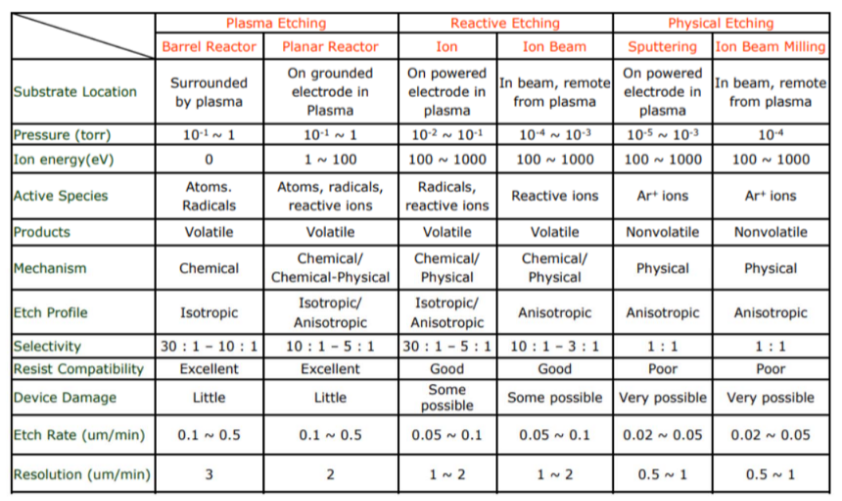
\includegraphics[width=0.75\textwidth,height=\textheight]{rie_etching_possibilities.png}
\caption{{rie} etching possibilities}\label{fig:enter-label}
}
\end{figure}

There is two categories of {rie} etching:

\begin{enumerate}
\def\labelenumi{\arabic{enumi}.}
\item
  \ul{Ion-Induced {rie}:} reaction controlled etching with typically
  \(Cl_2/Si\)

  \begin{itemize}
  \item
    When subststrate is not spontaneously etched away
  \item
    Ions modify the surface reactions in one way or another. Make the
    radicals to react with the substrate.
  \end{itemize}
\item
  \ul{Ion-Inhibitor {rie}:} desorption-controlled etching with typically
  \(F/Si, Cl_2/Al\).

  \begin{itemize}
  \item
    Substrate is etched spontaneously so we need an inhibiting layers to
    achieve directionality.
  \item
    The bottom of the trench is exposed to ion bombardment.
  \end{itemize}
\end{enumerate}

\hypertarget{fluorine-based-plasma---anisotropic-si-etching}{%
\paragraph{Fluorine-Based Plasma - Anisotropic Si
etching}\label{fluorine-based-plasma---anisotropic-si-etching}}

Due to the isotropic nature of the chemical reaction, we have to use
some inhibitor layer composed of Silicium, Fluor and oxygen. This is
some ion-inhibitor process and the oxygen covers the silicon surface
with silicon oxide. The issue is that the SF5+ will etch the layer
making it possible for the F* radicals to etch the silicon substrate.

\hypertarget{chlorine-based-plasma---thin-film-al-dry-etching}{%
\paragraph{Chlorine-Based Plasma - Thin-film Al Dry
etching}\label{chlorine-based-plasma---thin-film-al-dry-etching}}

Aluminum is spontaneously etched by \(Cl_2\) but there is a native
aluminum oxide layer. We have to use some ion bombardment because it is
essential for aluminum.

\hypertarget{chlorine-based-plasma---poly-si-dry-etching}{%
\paragraph{Chlorine-Based Plasma - Poly-Si Dry
etching}\label{chlorine-based-plasma---poly-si-dry-etching}}

We use som ion-induced {rie} with gases like \(Cl_2, HBr, O_2\).

\hypertarget{ion-milling-etching-thin-film-platinum-etching}{%
\paragraph{Ion Milling Etching: thin film platinum
etching}\label{ion-milling-etching-thin-film-platinum-etching}}

We use some \(Ar\) gas and the platinum has been \emph{physically}
etched by argon plasma. We can witness some sort of fence because the
platinum may redeposit on the sidewall creating some fences.

\hypertarget{inductively-coupled-plasma-rie}{%
\paragraph{\texorpdfstring{Inductively coupled Plasma
{rie}}{Inductively coupled Plasma rie}}\label{inductively-coupled-plasma-rie}}

Here we use some {ccp} to etch the silicon and other material slowly.
{icp} {rie} generates the plasma through a RF powered magnetic field
which allows us to create some very high plasma density.

\begin{figure}
\hypertarget{fig:enter-label}{%
\centering
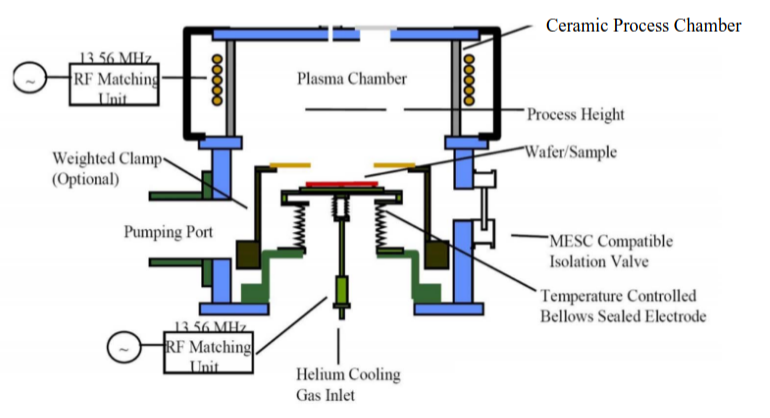
\includegraphics[width=0.75\textwidth,height=\textheight]{Setup_plasma_rie.png}
\caption{Plasma coupld {rie}}\label{fig:enter-label}
}
\end{figure}

\hypertarget{drie}{%
\subsubsection{\texorpdfstring{{drie}}{drie}}\label{drie}}

We also use some {drie} or Bosh process that allows us to draw some
pretty precise features with a high-aspect ratio (20-50), it is a cyclic
process where we alternate between etching and depositing. We etch using
some \(SF_6\) and deposit some polymer layer of \(C_4F_8\). We can etch
over \(10 \mu m/min\) and go through the whole wafer. We pulse but it
will still eat a bit of the sidewall. It is pretty good for MEMS
devices.

\hypertarget{etch-lag}{%
\paragraph{Etch Lag}\label{etch-lag}}

A bigger opening will etch more vertically compared to a shallower one
with the same amount of cycles.

\hypertarget{comparing-dry-etching}{%
\subsubsection{Comparing Dry etching}\label{comparing-dry-etching}}

\begin{longtable}[]{@{}ll@{}}
\caption{Etching Pressure Ranges}\tabularnewline
\toprule\noalign{}
\textbf{Etching Mode} & \textbf{Pressure (Torr)} \\
\midrule\noalign{}
\endfirsthead
\toprule\noalign{}
\textbf{Etching Mode} & \textbf{Pressure (Torr)} \\
\midrule\noalign{}
\endhead
\bottomrule\noalign{}
\endlastfoot
Ion Milling & \(10^{-4}\) -- \(10^{-3}\) \\
Reactive Ion Etching/Ion Milling & \(10^{-3}\) -- \(10^{-1}\) \\
Plasma Etching & \(10^{-1}\) -- \(5\) \\
\end{longtable}

\hypertarget{interconnects-al-cu-cmp}{%
\section{Interconnects, Al, Cu, CMP}\label{interconnects-al-cu-cmp}}

Interconnect is a crucial part of any IC's as they connect the various
transistors among each other and to connect the IC with other
components.

We first considered Aluminum for interconnect as it is cheap, compatible
with Si technology, it adheres well to SiO2. One major flaw is the low
melting point of 577 c.~Copper was for a long time avoided as it
diffuses really fast in Si and SiO2 and adheres not really well to SiO2.

\hypertarget{aluminum-as-interconnect}{%
\subsection{Aluminum as interconnect}\label{aluminum-as-interconnect}}

\hypertarget{spiking-and-pitting}{%
\subsubsection{Spiking and pitting}\label{spiking-and-pitting}}

Silicon will naturally diffuses non-uniformly into Aluminum creating
\textbf{spiking}, this Silicon that diffuses will leave some space that
the Aluminum will "\emph{fall}" into it due those pits.

Those pits could break some junction inside of a transistor.

\hypertarget{solution}{%
\paragraph{Solution}\label{solution}}

Add some Silicon to the Aluminum or during the PVD step. We can also add
some barrier metrial as Titanium-Tungsten.

\begin{figure}
\hypertarget{fig:TiW-label}{%
\centering
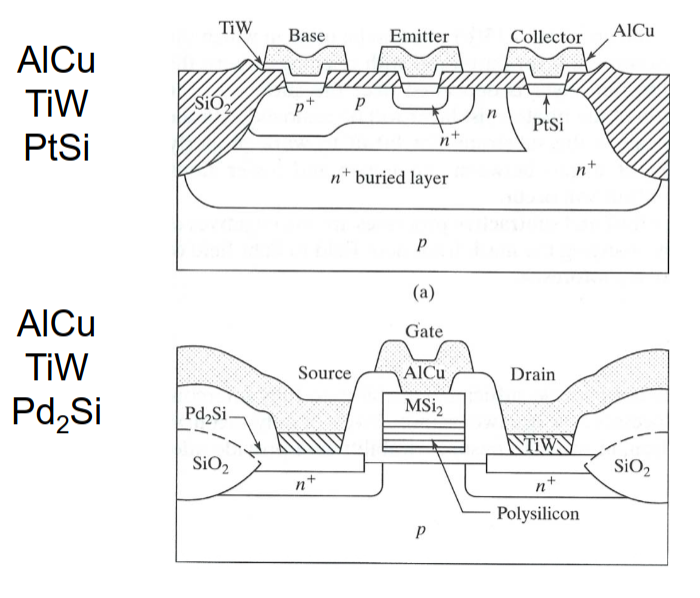
\includegraphics[width=0.5\textwidth,height=\textheight]{Solution_tiw.png}
\caption{Barrier solution to TiW}\label{fig:TiW-label}
}
\end{figure}

\hypertarget{silicides}{%
\paragraph{Silicides}\label{silicides}}

Silicium can react with various metal which have various resistivity and
can appear at different conditions. Those properties can be used to make
some metal to react with the wafer, the rest of the metal that didn't
react with the silicium.

\hypertarget{electromigration}{%
\subsubsection{Electromigration}\label{electromigration}}

If we make the interconnect too thin we can witness electrons carrying
away some chunk of metal. Also good to remember that the flow of current
is opposite to the flow of electrons.

\hypertarget{solution-1}{%
\paragraph{Solution}\label{solution-1}}

We can add Cu to Al, 95 \% Aluminum, 4\% copper and 1\% Silicon. Or the
simple solution is to use some Cu.

\hypertarget{multilevel-metal-problem}{%
\subsubsection{Multilevel Metal
Problem}\label{multilevel-metal-problem}}

We will have non planar structure in our wafer with all those layers and
structures we form. We will have some \textbf{via-depth} problem.

\hypertarget{solution-2}{%
\paragraph{Solution}\label{solution-2}}

This is why we usually make the contact wider and wider contacts as the
stack increase. We can also slightly shift the stacking to avoid
alignment issues.

We also have developed techniques to make the structure more planar by
filling up via with tungsten through {cvd} and we also deposit some
Aluminum using {pvd}. The filling of tungsten is a \emph{selective
deposition} as seen with the reaction:

\[2 WF_6 (g) + 3 Si (s) \longrightarrow 2 W (s) + 3SiF_4 (g)\]

\begin{figure}
\hypertarget{fig:enter-label}{%
\centering
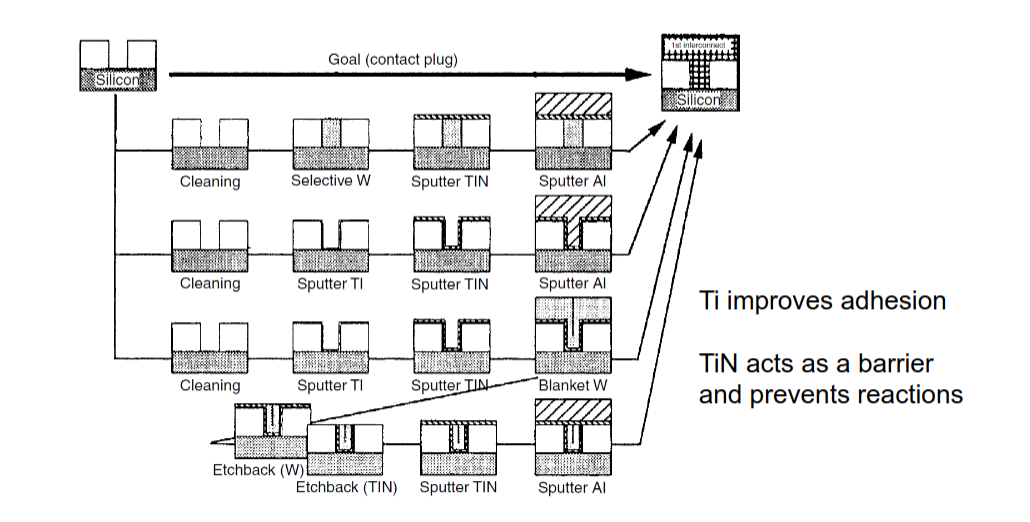
\includegraphics[width=0.75\textwidth,height=\textheight]{contact.png}
\caption{Several ways to create interlayer
contacts}\label{fig:enter-label}
}
\end{figure}

\hypertarget{cmp}{%
\subsubsection{\texorpdfstring{{cmp}}{cmp}}\label{cmp}}

\hypertarget{planirize-the-surface}{%
\paragraph{Planirize the surface}\label{planirize-the-surface}}

A common used techniques is to use oxide-{cmp} to planirize the surface
after applying some contacts. Then we can build on top of a flat and
clean surface.

Another way is to use some {cmp} that uses a \textbf{chemo-mechanical
polish}. It can be used to:

\begin{enumerate}
\def\labelenumi{\arabic{enumi}.}
\item
  Smoothing
\item
  Planarization: ideal after applying some interconnect
\item
  Damascene: a commonly used techniques in Cu interconnet and allows to
  draw some precise features
\end{enumerate}

\hypertarget{cmp-principle}{%
\paragraph{\texorpdfstring{{cmp}
principle}{cmp principle}}\label{cmp-principle}}

\begin{figure}
\hypertarget{fig:enter-label}{%
\centering
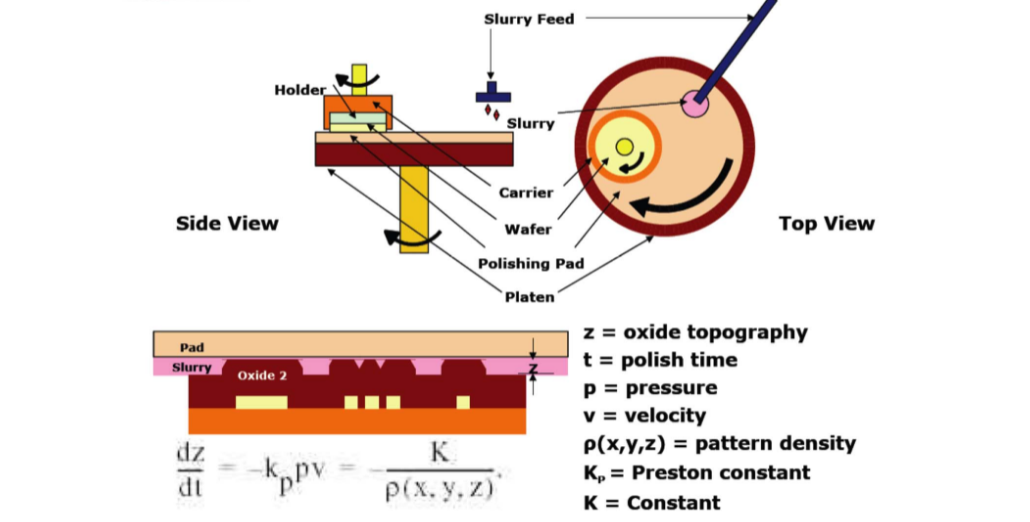
\includegraphics[width=0.75\textwidth,height=\textheight]{cmp_lucent.png}
\caption{{cmp} principle}\label{fig:enter-label}
}
\end{figure}

It is a pretty staight-forward process, we can also have some
\emph{multiwafer} machinery that allows us to process multiple wafer in
parallel.

This process is not perfect and can smooth out \emph{local} planarity
but it will distribute it \emph{globally} resulting to global
non-planarity which is not really the desired effect.

\hypertarget{solution-to-reach-global-planarity}{%
\paragraph{Solution to reach global
planarity}\label{solution-to-reach-global-planarity}}

\begin{figure}
\hypertarget{fig:enter-label}{%
\centering
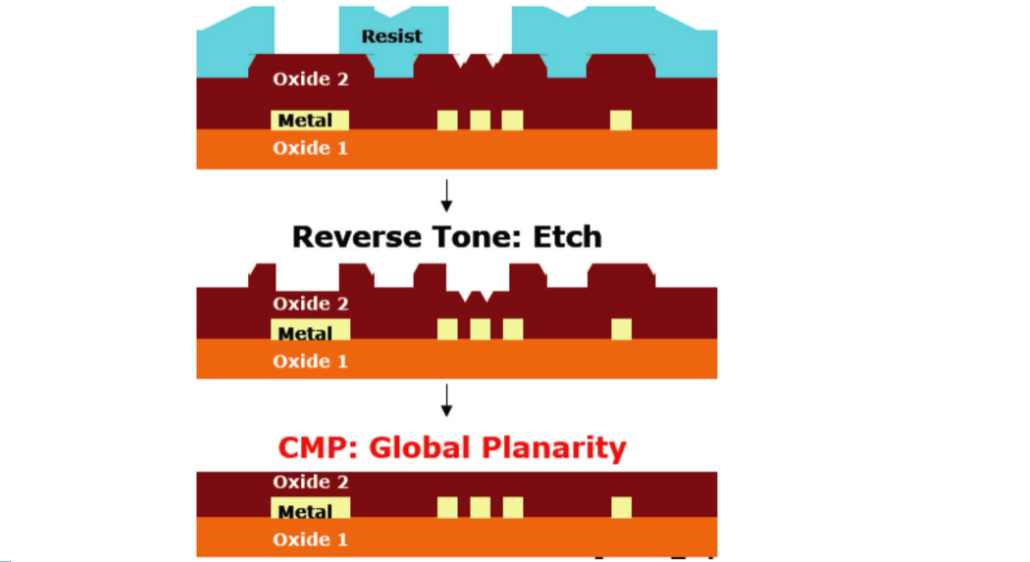
\includegraphics[width=0.65\textwidth,height=\textheight]{global_planarity.png}
\caption{Global planarity}\label{fig:enter-label}
}
\end{figure}

Another solution would be to add dummy oxide which will make the {cmp}
smoother. This dummy oxide can sometimes be seen in finished products.

\hypertarget{copper-ic}{%
\subsubsection{Copper IC}\label{copper-ic}}

The main reason to push for copper interconnect, is to further reduce
the delay time as we scale down.

\begin{figure}
\hypertarget{fig:enter-label}{%
\centering
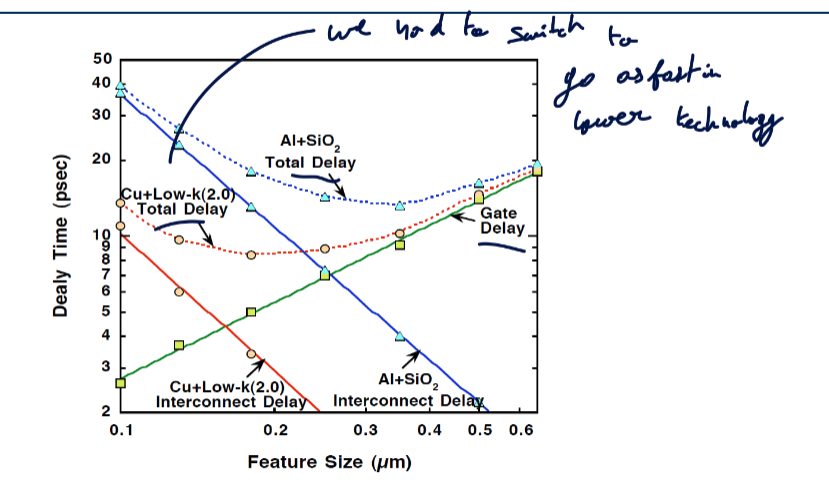
\includegraphics[width=0.5\textwidth,height=\textheight]{copper_ic.png}
\caption{Copper interconnect}\label{fig:enter-label}
}
\end{figure}

It also has some better resistance against failure but it doesn't adhere
well to dielectric, it diffuses with the dielectric. It is compatible
with tungsten plug (good point) but the copper just contaminate the chip
and the equipment, ...

So to avoid this, we will use some \emph{seed layer} that behaves as a
sort of protective layer. The damascene process is extensively used to
produce some pretty flat result.

\begin{figure}
\hypertarget{fig:enter-label}{%
\centering
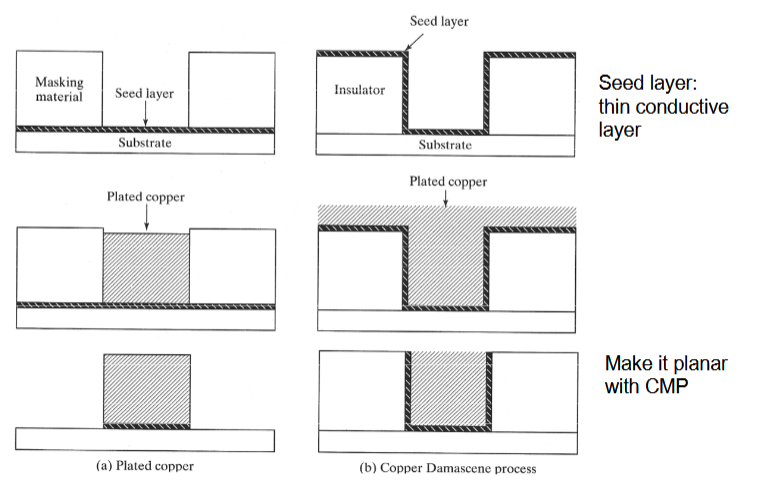
\includegraphics[width=0.5\textwidth,height=\textheight]{electroplating.png}
\caption{Copper, electroplating}\label{fig:enter-label}
}
\end{figure}

\hypertarget{damascene-process}{%
\paragraph{Damascene process}\label{damascene-process}}

r0.24
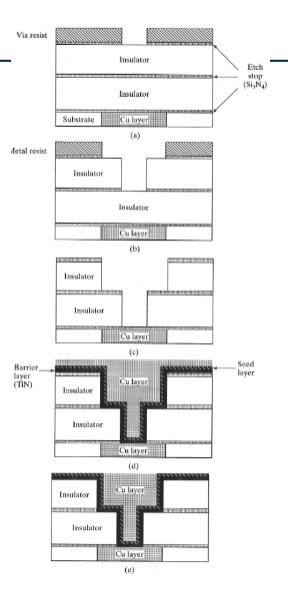
\includegraphics[width=0.9\textwidth,height=\textheight]{dual_damascene.png}

The idea behind this process, is to simply add this protective layer
(through {ald}), deposit the copper and polish using {cmp}.

The dual damascene process is extensively used in vias and interconnect
traces as it can make some thicker top traces

It is the de facto standard in CMOS processing. This allows to create
complex stack with many many layers.

If we are using the simple platting of copper, we can use some lift-off
process which makes removing the excedant of copper quite easy. Employed
especially for and .

\hypertarget{ic-processing-overview}{%
\section{IC Processing overview}\label{ic-processing-overview}}

\hypertarget{cmos}{%
\subsection{CMOS}\label{cmos}}

\begin{figure}
\hypertarget{fig:enter-label}{%
\centering
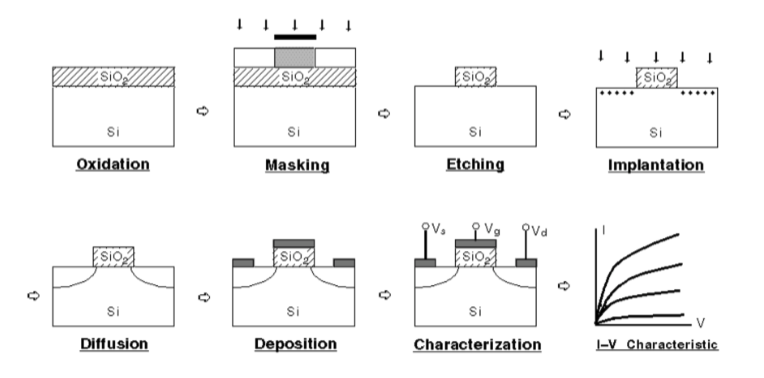
\includegraphics[width=0.5\textwidth,height=\textheight]{simplified_CMOS.png}
\caption{The simplified CMOS processing}\label{fig:enter-label}
}
\end{figure}

In the beginning, we used a lot of gate to control the gate which was a
sensible choice given the easy of connection and we just have some
thermal diffusion. But the biggest issue and limitation was the fact
that it was not a \textbf{self-aligned process}. Meaning that engineer
had to take margin when doing the gate creating some unnecessary overlap
which amplified the junction capacitance further reducing the speed. On
top of this, after applying we couldn't do a lot of other processes that
works at higher temperature !

In Aluminium process, we first dope through some high temperature step
then we need to align the gate on top of the source and drain.

But now, in poly-gate, we can whistand higher temperature and here we
use the poly gate as the mask for the source and drain region.
\textbf{The gate comes first, forcing the source and drain to be at the
right place}.

\hypertarget{self-alignment}{%
\subsubsection{Self-alignment}\label{self-alignment}}

\begin{figure}
\hypertarget{fig:enter-label}{%
\centering
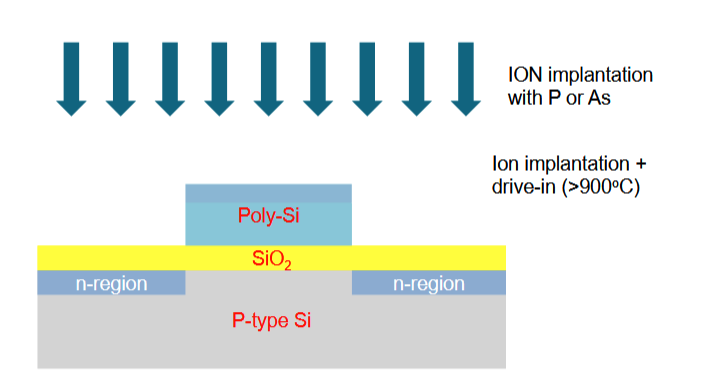
\includegraphics[width=0.5\textwidth,height=\textheight]{self_alignment_poly.png}
\caption{Self-alignment polygate}\label{fig:enter-label}
}
\end{figure}

\hypertarget{basic-flow}{%
\subsubsection{Basic flow}\label{basic-flow}}

We first start "drawing" the poly-silicon gate using a mask. We do for
the NMOS and PMOS at the same time. Once it is done, we remove the
photoresist, do some Boron implantation for NMOS. We implant some
Arsenic with low-energy (so we don't put too many) which acts like a
channel stop, to avoid any charges during operation to flow from a NMOS
to PMOS.

\begin{figure}
\hypertarget{fig:enter-label}{%
\centering
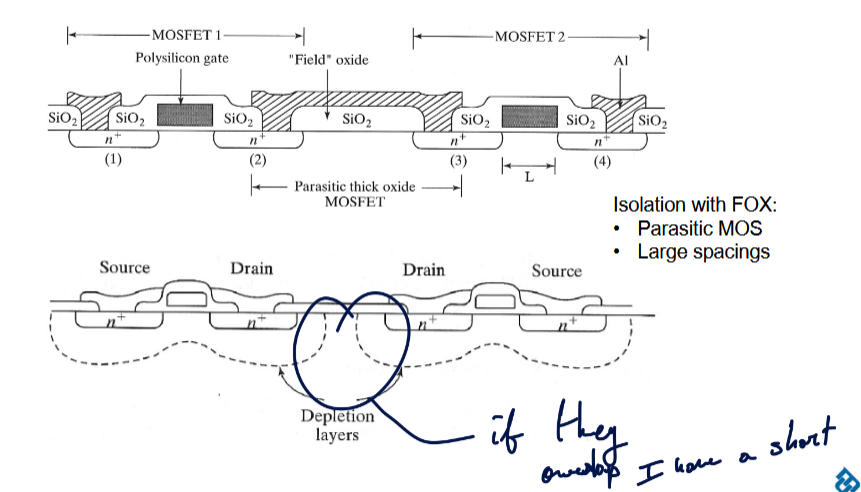
\includegraphics[width=0.5\textwidth,height=\textheight]{parasitic_NMOS.png}
\caption{Parasitic NMOS thick}\label{fig:enter-label}
}
\end{figure}

In this process step, we can find back the {locos} process and see the
appearance of those bird's beak. Then we apply remove the Nitride to
implant some Boron for the PMOS.

Once we have the desired region for the channel, we can add the
polysilicon and \textbf{then} the actual doping with some high dose
boron for PMOS and high dose phosphorus for NMOS. We just have to invert
the mask from the previous step. It is self-aligning since the
implantation will slightly bend around the gate which will create a
controlled channel capacitance.

Finally, we can do some {cvd} deposition of the contact holes and finish
it with some nice metallization and etching. And voilà ! we have a CMOS.
Ofc, it is not flat and nice as depicted in schematics. It is quite
chaotic and uneven.

\hypertarget{latch-up}{%
\paragraph{Latch-up}\label{latch-up}}

One big enemy: Latch-up ! Typically there is some undesired bipolar
junction that forms a \emph{thyristor}. So for this we usually use some
{epi} and {sti} to ensure no such behavior can occur.

\begin{figure}
\hypertarget{fig:enter-label}{%
\centering
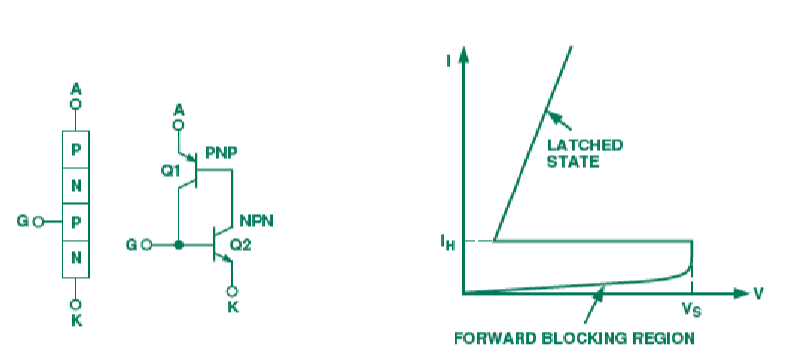
\includegraphics[width=0.5\textwidth,height=\textheight]{thyristor_operation.png}
\caption{Thyristor and its operation}\label{fig:enter-label}
}
\end{figure}

\begin{figure}
\hypertarget{fig:enter-label}{%
\centering
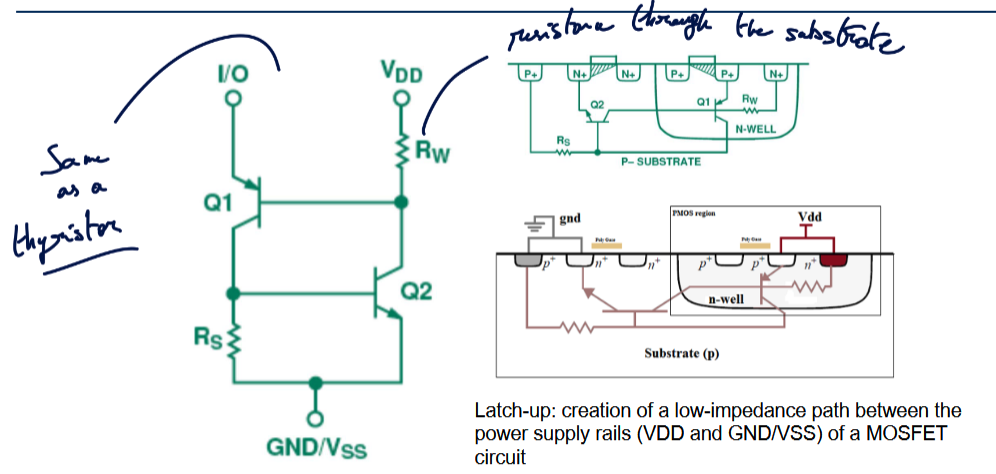
\includegraphics[width=0.5\textwidth,height=\textheight]{latchup.png}
\caption{Latch-up}\label{fig:enter-label}
}
\end{figure}

So this is why we love {sti} in this case !

\hypertarget{advanced-cmos-process}{%
\subsubsection{Advanced CMOS process}\label{advanced-cmos-process}}

We use a base substrate p where we grow some {epi} on top, we then
depose some with a buffer layer made of nitride. We use some plasma
etching to create trenches using the inverse of the active area mask.

\begin{figure}
\hypertarget{fig:enter-label}{%
\centering
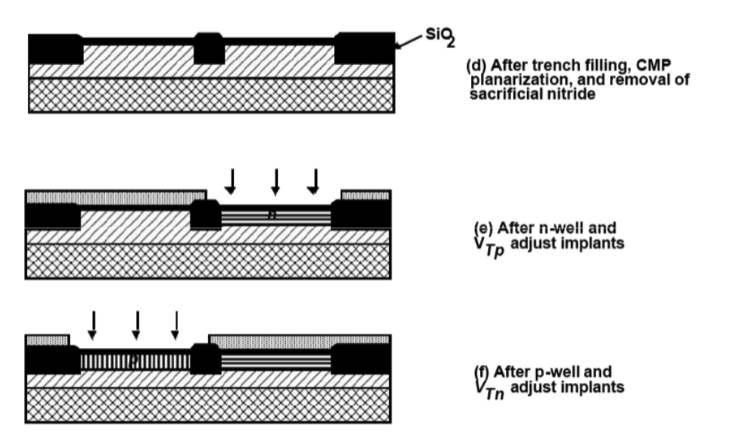
\includegraphics[width=0.5\textwidth,height=\textheight]{advanced_cmos.png}
\caption{Advanced CMOS process}\label{fig:enter-label}
}
\end{figure}

But this isn't always enough and sometimes, we need to do some {ldd} to
avoid \emph{hot electron} effect. This effect can sometimes change the
actual doping which can then destroy the junction and make MOS not work
at all !

\hypertarget{hot-carrier-effect}{%
\paragraph{Hot carrier effect}\label{hot-carrier-effect}}

It happens when a strong EM field is applied and when an electron has
enough \emph{kinetic energy} to break lattice bonds and hence create
another electron-hole pair. They have an energy over \(kT\). This will
increase the current in the channel but the holes will be absorbed by
the substrate creating a little current that can be monitored. This
creates a sort of BJT.

This is why we often add some spacer to help with this effect.

\hypertarget{salicide}{%
\subsubsection{Salicide}\label{salicide}}

It allows a better current flow synonym of more freedom in the layout !

\begin{figure}
\hypertarget{fig:enter-label}{%
\centering
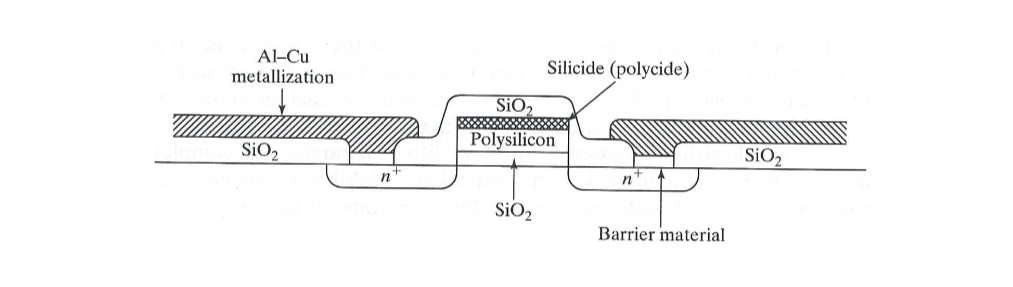
\includegraphics[width=0.5\textwidth,height=\textheight]{polycide_salicide.png}
\caption{Polycide - Salicide}\label{fig:enter-label}
}
\end{figure}

Salicides are \textbf{Self Aligned Silicides} hence the name. it
consists of:

\begin{enumerate}
\def\labelenumi{\arabic{enumi}.}
\item
  metal deposition;
\item
  annealing forms silicide on polysilicon gate and single-crystal
  silicon source/drain areas
\item
  Unreacted metal is selectively etched away.
\end{enumerate}

\begin{figure}
\hypertarget{fig:enter-label}{%
\centering
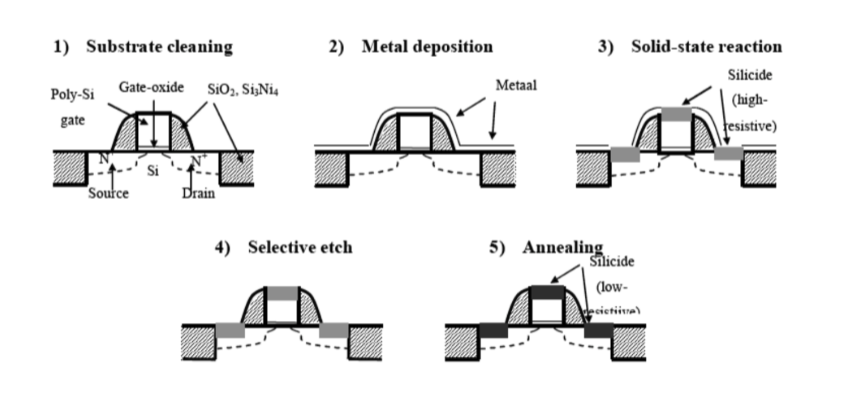
\includegraphics[width=0.5\textwidth,height=\textheight]{salicide.png}
\caption{Salicide}\label{fig:enter-label}
}
\end{figure}

As we get lower and lower, we need to use {ald} to realize this
technique.

\begin{figure}
\hypertarget{fig:enter-label}{%
\centering
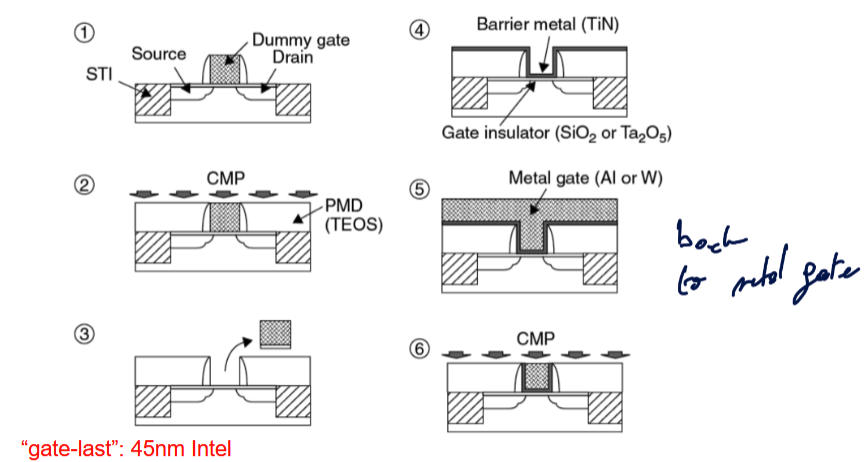
\includegraphics[width=0.5\textwidth,height=\textheight]{gate_MOSFET.png}
\caption{Gate MOSFET}\label{fig:enter-label}
}
\end{figure}

\hypertarget{guest-lecture}{%
\section{Guest Lecture}\label{guest-lecture}}

\hypertarget{glossary}{%
\section{Glossary}\label{glossary}}

\begin{itemize}
\tightlist
\item
  Mean Free Path (MFP):

  \begin{itemize}
  \tightlist
  \item
    The average distance a particle (such as an electron, atom, or
    molecule) travels between collisions. In semiconductors and thin
    films, it influences transport phenomena.
  \end{itemize}
\item
  Chemical Vapor Deposition (CVD):

  \begin{itemize}
  \tightlist
  \item
    A process where gaseous precursors chemically react or decompose on
    a substrate surface to form a solid material, often used for
    thin-film fabrication in semiconductor manufacturing.
  \end{itemize}
\item
  Physical Vapor Deposition (PVD):

  \begin{itemize}
  \tightlist
  \item
    A vacuum-based process in which material is physically vaporized and
    deposited onto a substrate to form thin films.
  \end{itemize}
\item
  Molecular Beam Epitaxy (MBE):

  \begin{itemize}
  \tightlist
  \item
    An ultra-high vacuum technique where atomic or molecular beams are
    directed at a heated substrate to grow highly controlled epitaxial
    layers.
  \end{itemize}
\item
  Atomic Layer Deposition (ALD):

  \begin{itemize}
  \tightlist
  \item
    A vapor-phase technique for depositing thin films one atomic layer
    at a time using sequential, self-limiting reactions. Offers
    excellent conformality.
  \end{itemize}
\item
  Shallow Trench Isolation (STI):

  \begin{itemize}
  \tightlist
  \item
    A process used to isolate CMOS transistors on a silicon wafer by
    etching shallow trenches and filling them with dielectric material.
  \end{itemize}
\item
  Deep Trench Isolation (DTI):

  \begin{itemize}
  \tightlist
  \item
    An isolation method using deep etched trenches filled with
    insulators, used in 3D integration and high-voltage devices.
  \end{itemize}
\item
  LOCal Oxidation of Silicon (LOCOS):

  \begin{itemize}
  \tightlist
  \item
    A technique for selectively growing oxide on silicon for isolation
    by locally exposing regions to thermal oxidation.
  \end{itemize}
\item
  TEtraethylorthOSilicate (TEOS):

  \begin{itemize}
  \tightlist
  \item
    A silicon precursor used in CVD to deposit silicon dioxide films.
    TEOS provides good conformality and uniformity.
  \end{itemize}
\item
  Chemical-Mechanical Polishing (CMP):

  \begin{itemize}
  \tightlist
  \item
    A planarization process combining chemical slurry and mechanical
    abrasion to produce flat surfaces in semiconductor fabrication.
  \end{itemize}
\item
  Low-temperature Oxidation (LTO):

  \begin{itemize}
  \tightlist
  \item
    A thermal oxidation process performed at lower temperatures to form
    silicon dioxide, used when high-temperature processing is not
    feasible.
  \end{itemize}
\item
  High-temperature Oxidation (HTO):

  \begin{itemize}
  \tightlist
  \item
    An oxidation process performed at high temperatures to produce
    high-quality oxide films on silicon.
  \end{itemize}
\item
  Plasma Enhanced CVD (PECVD):

  \begin{itemize}
  \tightlist
  \item
    A variant of CVD where plasma is used to enhance chemical reactions,
    enabling deposition at lower temperatures.
  \end{itemize}
\item
  Low Pressure CVD (LPCVD):

  \begin{itemize}
  \tightlist
  \item
    A CVD process carried out under reduced pressure, leading to better
    uniformity and fewer contaminants.
  \end{itemize}
\item
  Anti Reflective Coating (ARC):

  \begin{itemize}
  \tightlist
  \item
    A thin film applied to reduce reflections and improve pattern
    fidelity in photolithography.
  \end{itemize}
\item
  Rapid Thermal Annealing (RTA):

  \begin{itemize}
  \tightlist
  \item
    A process of quickly heating wafers to activate dopants or repair
    damage without significantly affecting the rest of the structure.
  \end{itemize}
\item
  Secondary Ion eMission Spectroscopy (SIMS):

  \begin{itemize}
  \tightlist
  \item
    An analytical technique that sputters a sample surface and detects
    secondary ions to determine composition and depth profiles.
  \end{itemize}
\item
  Spreading Resistance Profilometry (SRP):

  \begin{itemize}
  \tightlist
  \item
    A technique for measuring the resistivity and doping profile of
    semiconductors by placing probes along a beveled surface.
  \end{itemize}
\item
  Reactive Ion Etching (RIE):

  \begin{itemize}
  \tightlist
  \item
    A plasma-based etching technique using reactive gases to
    anisotropically etch materials with fine resolution.
  \end{itemize}
\item
  Deep Reactive Ion Etching (DRIE):

  \begin{itemize}
  \tightlist
  \item
    An advanced RIE process capable of etching deep, high-aspect-ratio
    features, especially in MEMS and silicon micromachining.
  \end{itemize}
\item
  Capacitively Coupled Plasma (CCP):

  \begin{itemize}
  \tightlist
  \item
    A plasma generation method used in etching where power is
    capacitively coupled through electrodes. Often used in RIE.
  \end{itemize}
\item
  Inductively Coupled Plasma (ICP):

  \begin{itemize}
  \tightlist
  \item
    A high-density plasma source where power is inductively coupled
    through coils, providing high etch rates and better control.
  \end{itemize}
\item
  Epitaxy (EPI):

  \begin{itemize}
  \tightlist
  \item
    The process of epitaxy allows the growth of a higher purity layer on
    a substrate of the same material. The goal of the epitaxy process is
    to make electron transmission more effective through the device.
  \end{itemize}
\end{itemize}

\end{document}
